\chapter{Resultados}
\label{cap:resultados}

% ------------------------------------------------------------------------------
\section{Pré-tratamento dos dados}
\label{sec:res-pretratamento}
% ------------------------------------------------------------------------------

O painel principal reúne 2.234 pregões por instituição, de 02/10/2017 a
30/09/2026, e o painel de extensão, 1.690, de 02/01/2019 a 13/10/2025. O
primeiro pregão de cada janela não tem fechamento anterior e, portanto,
volatilidade estimada, de modo que os painéis finais têm 2.233 e 1.689
observações (15.631 e 13.512 valores). A verificação de consistência do OHLC,
com tolerância de $10^{-6}$, não encontra violação em nenhuma série. O filtro
de liquidez remove um único pregão, o do Banco Pan em 15/01/2019, e nenhum no
painel principal. A regra de variância nula trata como ausentes 14 valores no
painel principal (0,09\%) e 13 no de extensão (0,10\%), no máximo seis por
instituição. Esses valores, mais os dois que o filtro de liquidez torna
ausentes no painel de extensão (o pregão de 15/01/2019 e o seguinte, que fica
sem fechamento anterior), são os únicos imputados pelo filtro de Kalman: 14 no
painel principal e 15 no de extensão (0,09\% e 0,11\%;
Tabela~\ref{tab:pretratamento}).

Os retornos extremos ($|z|>5$) somam 53 observações em cada painel, em 24
datas no principal e em 20 no de extensão. Trinta e sete e 41 delas,
respectivamente, em oito datas de março e abril de 2020 (as mesmas nos dois
painéis), ocorrem em duas ou mais instituições no mesmo dia e são
classificadas como eventos sistêmicos. As demais, 16 e 12, são casos isolados,
listados nas Tabelas~\ref{tab:outliers-a} e~\ref{tab:outliers-b}. Para 17 dos 18 casos distintos há fonte datada
que registra o evento ou o contexto do dia e para um (BPAC11 em 23/03/2020) a causa não
foi identificada. Nenhuma observação é removida ou winsorizada.

\begin{table}[H]
\centering
\caption{Pré-tratamento por instituição e por painel}
\label{tab:pretratamento}
\begin{tabular}{lccccc}
\toprule
Instituição & Abaixo do piso & Variância nula & Imputados & $|z|>5$ & Isolados \\
\midrule
\multicolumn{6}{l}{\textit{Painel principal (N = 7)}} \\
ITUB4  & 0 &  0 &  0 &  4 &  0 \\
BBDC4  & 0 &  0 &  0 &  8 &  3 \\
BBAS3  & 0 &  1 &  1 & 11 &  3 \\
SANB11 & 0 &  3 &  3 &  7 &  1 \\
BPAC11 & 0 &  1 &  1 & 10 &  5 \\
BRSR6  & 0 &  3 &  3 &  8 &  4 \\
ABCB4  & 0 &  6 &  6 &  5 &  0 \\
Total  & 0 & 14 & 14 & 53 & 16 \\
\midrule
\multicolumn{6}{l}{\textit{Painel de extensão (N = 8)}} \\
ITUB4  & 0 &  0 &  0 &  4 &  0 \\
BBDC4  & 0 &  0 &  0 &  8 &  3 \\
BBAS3  & 0 &  1 &  1 & 11 &  3 \\
SANB11 & 0 &  2 &  2 &  6 &  0 \\
BPAC11 & 0 &  1 &  1 &  8 &  3 \\
BRSR6  & 0 &  3 &  3 &  5 &  1 \\
ABCB4  & 0 &  4 &  4 &  5 &  0 \\
BPAN4  & 1 &  2 &  4 &  6 &  2 \\
Total  & 1 & 13 & 15 & 53 & 12 \\
\bottomrule
\end{tabular}
\legend{Fonte: elaboração própria. Em BPAN4, os quatro valores imputados são os
dois de variância nula, o pregão de 15/01/2019, filtrado por liquidez, e o
seguinte, sem fechamento anterior.}
\end{table}

\begin{table}[H]
\centering
\footnotesize
\caption{Retornos extremos isolados ($|z|>5$ em uma única instituição), 2017--2020}
\label{tab:outliers-a}
\begin{tabular}{llrcp{6.8cm}}
\toprule
Banco & Data & Retorno (\%) & Painéis & Evento (fonte) \\
\midrule
BRSR6 & 04/10/2017 & $-11{,}51$ & 7 & Fato relevante do governo do RS anuncia a venda de parte das ações do Banrisul; as preferenciais caem mais de 10\% no dia \parencite{extraclasse2017, tribunapr2018} \\
BRSR6 & 08/10/2018 & $11{,}06$ & 7 & Pregão seguinte ao primeiro turno das eleições; o Ibovespa sobe 4,57\% e as estatais lideram a alta (a fonte não cita o Banrisul) \parencite{seudinheiro2018} \\
BPAN4 & 22/05/2019 & $20{,}96$ & 8 & Anúncio de plano de conta digital e relatório da Empiricus recomendando a compra; a ação fecha em alta de 23,3\% \parencite{seudinheiro2019pan} \\
BPAC11 & 23/08/2019 & $-16{,}48$ & 7 e 8 & Banco é alvo da 64ª fase da Lava Jato (busca e apreensão); as \textit{units} caem 15,2\% \parencite{moneytimes20190823} \\
BPAC11 & 26/08/2019 & $-20{,}43$ & 7 e 8 & Reportagem do site O Antagonista sobre suposto esquema de lavagem de dinheiro no banco; as \textit{units} caem 18,5\% \parencite{seudinheiro20190826} \\
BPAC11 & 27/08/2019 & $16{,}02$ & 7 e 8 & Recuperação parcial após queda de 31\% nos dois pregões anteriores \parencite{moneytimes20190827} \\
BRSR6 & 10/03/2020 & $13{,}98$ & 7 e 8 & Recuperação do Ibovespa (+7,14\%) após a queda de 12,19\% de 09/03 \parencite{suno20200311, infomoney2020cb} \\
BPAC11 & 11/03/2020 & $-14{,}34$ & 7 & OMS caracteriza a COVID-19 como pandemia; o Ibovespa cai 7,64\% e a B3 aciona o \textit{circuit breaker} \parencite{moneytimes20200311} \\
BPAC11 & 23/03/2020 & $-13{,}89$ & 7 & Causa não identificada \\
BBAS3 & 24/04/2020 & $-14{,}35$ & 7 e 8 & Demissão do ministro Sergio Moro; o Ibovespa cai 5,45\% e o BBAS3, 13,4\% \parencite{moneytimes20200424} \\
BPAN4 & 03/06/2020 & $19{,}09$ & 8 & Comunicado de 02/06/2020: o BTG informa a compra de 4,75 milhões de preferenciais (30,35\% das PN e 41,52\% do capital total); a ação já subira 15,7\% em 02/06 \parencite{pan2020comunicado} \\
\bottomrule
\end{tabular}
\legend{Fonte: elaboração própria. Retorno logarítmico diário, em pontos percentuais. Todos os casos permanecem na amostra. Um mesmo retorno pode ser sinalizado em um painel e não no outro, porque o escore $z$ usa a média e o desvio-padrão da janela de cada painel. A fonte registra o evento do dia (ou da véspera, no caso do Pan em 03/06/2020); a associação com o retorno é temporal e não foi testada. Continua na Tabela~\ref{tab:outliers-b}.}
\end{table}

\begin{table}[H]
\centering
\footnotesize
\caption{Retornos extremos isolados ($|z|>5$ em uma única instituição), 2021--2026}
\label{tab:outliers-b}
\begin{tabular}{llrcp{6.8cm}}
\toprule
Banco & Data & Retorno (\%) & Painéis & Evento (fonte) \\
\midrule
BBAS3 & 22/02/2021 & $-12{,}38$ & 7 e 8 & A troca do comando da Petrobras pelo governo gera temor de interferência em estatais; o BBAS3 cai 11,65\% \parencite{moneytimes20210222} \\
BBDC4 & 09/11/2022 & $-19{,}10$ & 7 e 8 & Resultado do 3T22 (lucro de R\$~5,2 bilhões, queda de 22,8\%); maior queda diária da ação em 24 anos \parencite{infomoney20221109} \\
BBDC4 & 07/02/2024 & $-17{,}32$ & 7 e 8 & Resultado do 4T23 abaixo do esperado e \textit{guidance} de 2024; a preferencial cai 15,7\% \parencite{moneytimes20240207} \\
BBDC4 & 08/05/2025 & $14{,}53$ & 7 e 8 & Resultado do 1T25 (lucro recorrente de R\$~5,9 bilhões, alta de 39\%); a ação sobe cerca de 15\% \parencite{moneytimes20250507, nord2025} \\
BBAS3 & 16/05/2025 & $-13{,}57$ & 7 e 8 & Resultado do 1T25 (lucro ajustado cai 20,7\%) e suspensão de parte do \textit{guidance}; a ação cai 12,7\% \parencite{moneytimes20250515, folhape2025} \\
BRSR6 & 14/04/2026 & $-11{,}83$ & 7 & BTG Pactual e UBS BB rebaixam a recomendação para venda; a ação cai 11,2\% \parencite{financenews20260414} \\
SANB11 & 31/07/2026 & $12{,}53$ & 7 & O Santander Espanha anuncia oferta voluntária de permuta com prêmio de 15\%; as \textit{units} sobem cerca de 13\% \parencite{investing20260731} \\
\bottomrule
\end{tabular}
\legend{Fonte: elaboração própria. Continuação da Tabela~\ref{tab:outliers-a}.}
\end{table}

% ------------------------------------------------------------------------------
\section{Propriedades das séries}
\label{sec:res-propriedades}
% ------------------------------------------------------------------------------

Após a regra de variância nula, a curtose em excesso da log-volatilidade
situa-se entre 1,8 e 4,2 nos dois painéis, e o menor valor de cada série está,
no máximo, a 7,5 desvios-padrão da média no painel principal (BPAC11) e a 6,1
no de extensão (BRSR6 e ABCB4; Tabela~\ref{tab:descritivas}).

\begin{table}[H]
\centering
\caption{Estatísticas descritivas da log-volatilidade anualizada}
\label{tab:descritivas}
\small
\begin{tabular}{lrrrrrr}
\toprule
Instituição & Média & DP & Mín. & Máx. & Assimetria & Curtose \\
\midrule
\multicolumn{7}{l}{\textit{Painel principal (N = 7)}} \\
ITUB4  & $-1{,}43$ & 0,46 & $-3{,}18$ & 1,03 &  0,37 & 1,77 \\
BBDC4  & $-1{,}34$ & 0,45 & $-2{,}93$ & 1,28 &  0,59 & 2,25 \\
BBAS3  & $-1{,}38$ & 0,51 & $-3{,}58$ & 1,37 &  0,50 & 2,07 \\
SANB11 & $-1{,}36$ & 0,48 & $-3{,}76$ & 1,23 &  0,18 & 2,42 \\
BPAC11 & $-1{,}09$ & 0,51 & $-4{,}90$ & 1,64 &  0,01 & 3,75 \\
BRSR6  & $-1{,}33$ & 0,48 & $-4{,}50$ & 0,86 & $-0{,}34$ & 4,16 \\
ABCB4  & $-1{,}39$ & 0,54 & $-4{,}73$ & 1,05 & $-0{,}67$ & 3,87 \\
\midrule
\multicolumn{7}{l}{\textit{Painel de extensão (N = 8)}} \\
ITUB4  & $-1{,}42$ & 0,47 & $-3{,}18$ & 1,03 &  0,43 & 1,80 \\
BBDC4  & $-1{,}34$ & 0,46 & $-2{,}93$ & 1,28 &  0,67 & 2,37 \\
BBAS3  & $-1{,}40$ & 0,51 & $-3{,}58$ & 1,37 &  0,64 & 2,22 \\
SANB11 & $-1{,}37$ & 0,48 & $-3{,}55$ & 1,23 &  0,30 & 2,26 \\
BPAC11 & $-1{,}05$ & 0,50 & $-3{,}13$ & 1,64 &  0,46 & 2,15 \\
BRSR6  & $-1{,}36$ & 0,46 & $-4{,}17$ & 0,86 &  0,07 & 3,24 \\
ABCB4  & $-1{,}36$ & 0,55 & $-4{,}73$ & 1,05 & $-0{,}68$ & 4,21 \\
BPAN4  & $-0{,}86$ & 0,54 & $-3{,}74$ & 1,44 & $-0{,}02$ & 1,74 \\
\bottomrule
\end{tabular}
\legend{Fonte: elaboração própria. Curtose em excesso.}
\end{table}

O ADF, o DF-GLS, o Phillips-Perron e o Zivot-Andrews rejeitam a raiz unitária
nas 15 séries dos dois painéis, e o KPSS rejeita a estacionariedade nas 15
(Tabela~\ref{tab:testes}). O Ljung-Box e o ARCH-LM rejeitam a ausência de
autocorrelação e de heterocedasticidade condicional ($p<0{,}0001$ em todas).
O parâmetro de integração fracionária fica entre 0,47 (BPAC11) e 0,60 (BBAS3)
no painel principal, com erro-padrão assintótico de 0,107, e entre 0,53 e 0,68
no de extensão, com erro-padrão de 0,116. No painel principal, cada estimativa
difere de zero (estatística de 4,4 a 5,6) e de um (3,8 a 4,9), e todas estão a
menos de um erro-padrão de 0,5. No de extensão, as estimativas diferem de zero
(4,6 a 5,9) e de um (2,8 a 4,0) e estão a menos de 1,6 erro-padrão de 0,5. As
séries estão, portanto, na fronteira entre a memória longa estacionária
($d<0{,}5$) e a não estacionária ($d\geq0{,}5$), sem serem nem $I(0)$ nem
$I(1)$. Isso reconcilia a rejeição simultânea do ADF e do KPSS e justifica a
estimação do VAR em níveis (Capítulo~\ref{cap:metodologia}).

\begin{table}[H]
\centering
\caption{Testes de estacionariedade e parâmetro de memória longa}
\label{tab:testes}
\small
\begin{tabular}{lcccccc}
\toprule
Instituição & ADF & KPSS ($p$) & DF-GLS & PP & ZA & $\hat{d}$ \\
\midrule
\multicolumn{7}{l}{\textit{Painel principal (N = 7), erro-padrão de $\hat{d}$: 0,107}} \\
ITUB4  & $-17{,}74$ & $<0{,}01$ & $-10{,}00$ & $-31{,}69$ & $-12{,}32$ & 0,495 \\
BBDC4  & $-19{,}31$ & $<0{,}01$ &  $-5{,}88$ & $-33{,}65$ & $-13{,}17$ & 0,528 \\
BBAS3  & $-17{,}82$ & $<0{,}01$ &  $-2{,}40$ & $-30{,}60$ & $-12{,}16$ & 0,599 \\
SANB11 & $-19{,}74$ & $<0{,}01$ &  $-9{,}31$ & $-34{,}01$ & $-13{,}23$ & 0,483 \\
BPAC11 & $-19{,}26$ & $<0{,}01$ & $-10{,}48$ & $-34{,}37$ & $-13{,}23$ & 0,474 \\
BRSR6  & $-22{,}88$ & $<0{,}01$ & $-12{,}37$ & $-37{,}15$ & $-14{,}61$ & 0,539 \\
ABCB4  & $-20{,}97$ & $<0{,}01$ &  $-9{,}76$ & $-35{,}40$ & $-15{,}57$ & 0,589 \\
\midrule
\multicolumn{7}{l}{\textit{Painel de extensão (N = 8), erro-padrão de $\hat{d}$: 0,116}} \\
ITUB4  & $-14{,}68$ & $<0{,}01$ &  $-7{,}72$ & $-26{,}41$ & $-12{,}06$ & 0,623 \\
BBDC4  & $-15{,}95$ & $<0{,}01$ &  $-9{,}38$ & $-27{,}89$ & $-11{,}91$ & 0,607 \\
BBAS3  & $-14{,}47$ & $<0{,}01$ &  $-6{,}69$ & $-24{,}90$ & $-10{,}24$ & 0,679 \\
SANB11 & $-16{,}29$ & $<0{,}01$ &  $-6{,}62$ & $-28{,}00$ & $-12{,}08$ & 0,533 \\
BPAC11 & $-15{,}08$ & $<0{,}01$ &  $-7{,}57$ & $-26{,}88$ & $-10{,}88$ & 0,677 \\
BRSR6  & $-19{,}33$ & $<0{,}01$ &  $-4{,}09$ & $-31{,}30$ & $-13{,}09$ & 0,533 \\
ABCB4  & $-17{,}62$ & $<0{,}01$ &  $-8{,}97$ & $-29{,}51$ & $-13{,}20$ & 0,667 \\
BPAN4  & $-15{,}38$ & $<0{,}01$ &  $-6{,}82$ & $-27{,}13$ & $-12{,}01$ & 0,602 \\
\bottomrule
\end{tabular}
\legend{Fonte: elaboração própria. Valores críticos a 5\%: ADF $-2{,}86$; DF-GLS
$-1{,}94$; PP $-2{,}86$; ZA $-5{,}08$. O KPSS reporta o limite inferior do
$p$-valor.}
\end{table}

A ordem do VAR é $p=2$ pela convenção da literatura. No painel principal, o
critério de Schwarz (BIC de $-13{,}536$) também a seleciona, com margem de
apenas 0,002 sobre $p=1$. O AIC escolheria $p=6$ e o HQ, $p=3$. No painel de
extensão, o BIC escolheria $p=1$ ($-15{,}588$, contra $-15{,}517$ para $p=2$),
o HQ seleciona $p=2$ e o AIC, $p=5$. O VAR é estável nos dois painéis (módulo
máximo das raízes de 0,828 e 0,865), e o Apêndice~\ref{ap:robustez} mostra que
o ranking dos bancos não depende de $p$.

% ------------------------------------------------------------------------------
\section{Seleção dos fatores de esquecimento}
\label{sec:res-kappa}
% ------------------------------------------------------------------------------

A Tabela~\ref{tab:grade-kappa} reporta a log-verossimilhança preditiva de cada
par $(\kappa_1,\kappa_2)$ no painel principal. O par selecionado é
$(0{,}995;\ 0{,}99)$, com peso posterior igual a 1, e é o mesmo no painel de
extensão. A folga é grande: o segundo melhor par, $(1{,}00;\ 0{,}99)$, que
corresponde a coeficientes constantes, fica 121,5 pontos abaixo no painel
principal e 148,2 no de extensão, e o melhor par estimável pelo pacote entre os
demais, $(0{,}99;\ 0{,}99)$, 219,1 e 209,6 pontos abaixo. A variação temporal
dos coeficientes melhora, portanto, a previsão um passo à frente, ainda que
$\kappa_1=0{,}995$ implique uma memória de cerca de 200 observações, bem mais
lenta que a da covariância ($\kappa_2=0{,}99$, cerca de 100 observações). 

\begin{table}[H]
\centering
\caption{Log-verossimilhança preditiva por par $(\kappa_1,\kappa_2)$ (painel principal)}
\label{tab:grade-kappa}
\begin{tabular}{lccc}
\toprule
 & $\kappa_2=0{,}94$ & $\kappa_2=0{,}96$ & $\kappa_2=0{,}99$ \\
\midrule
$\kappa_1=0{,}94$  & $-19.080$ & $-15.885$ & $-12.370$ \\
$\kappa_1=0{,}96$  & $-13.830$ & $-11.723$ &  $-9.321$ \\
$\kappa_1=0{,}98$  &  $-9.929$ &  $-8.671$ &  $-7.163$ \\
$\kappa_1=0{,}99$  &  $-8.445$ &  $-7.528$ &  $-6.410$ \\
$\kappa_1=0{,}995$ &  $-7.890$ &  $-7.125$ & $\mathbf{-6.191}$ \\
$\kappa_1=1{,}00$  &  $-7.694$ &  $-7.060$ &  $-6.312$ \\
\bottomrule
\end{tabular}
\legend{Fonte: elaboração própria. Soma de $\ell_t$ para $t>t_0=200$. Em negrito,
o par selecionado. Painel de extensão: mesmo vencedor, com log-verossimilhança de
$-5.271$.}
\end{table}

% ------------------------------------------------------------------------------
\section{Conectividade estática}
\label{sec:res-estatica}
% ------------------------------------------------------------------------------

Com $p=2$ e $\tau=10$, o índice de conectividade total da amostra completa é
de 52,9\% no painel principal e de 55,7\% no de extensão. Como o nível do
índice depende do número de instituições, não é comparado ao de outros estudos
nem entre os painéis (Capítulo~\ref{cap:metodologia}).

A Tabela~\ref{tab:dy} reúne TO, FROM e NET e o confronto com a segmentação do
Banco Central, ordenado pelo TO. No painel principal, os cinco primeiros do
ranking de transmissão são exatamente os cinco bancos do S1, o ABC Brasil vem em
sexto e o Banrisul, em sétimo. O Itaú é o maior transmissor líquido ($+19{,}3$),
seguido por Bradesco ($+8{,}9$) e Banco do Brasil ($+2{,}8$). Santander e BTG,
ambos do S1, são receptores líquidos ($-2{,}0$ e $-5{,}0$), e os maiores
receptores são Banrisul ($-14{,}9$) e ABC Brasil ($-9{,}2$). O TO varia de 28,6 a
81,0 e o FROM, de 43,4 a 61,7: o ranking é determinado pela transmissão. O par
mais intenso é Itaú-Bradesco: 18,5\% da variância do Itaú vem do Bradesco e
19,7\% da do Bradesco vem do Itaú.

No painel de extensão, os cinco primeiros do ranking são de novo os cinco do S1,
e todos são transmissores líquidos (Itaú $+18{,}4$, BTG $+5{,}1$, Bradesco
$+4{,}8$, Santander $+3{,}6$ e Banco do Brasil $+1{,}8$). Os receptores são
Banrisul ($-18{,}4$), ABC Brasil ($-9{,}5$) e Pan ($-5{,}8$). A posição do BTG
muda entre os painéis, de receptor líquido (NET de $-5{,}0$ e TO de 42,4) a
transmissor líquido (NET de $+5{,}1$ e TO de 61,2); a diferença acompanha a de
período e a inclusão do Pan e é mais uma razão para não comparar níveis entre
painéis. Na matriz do painel de extensão, 10,7\% da variância do Pan vem do BTG,
e 8,4\% da do BTG vem do Pan.

Nos dois painéis, a ordenação dos bancos pelo PageRank e pela centralidade de
autovetor é idêntica à ordenação pelo FROM, como discutido na Metodologia. O
Itaú é o maior transmissor líquido nas 13 especificações de robustez de cada
painel, e o Banrisul, o maior receptor em 12 delas no painel principal e em 11
no de extensão (Apêndice~\ref{ap:robustez}).

\begin{table}[H]
\centering
\caption{Conectividade direcional e segmentação prudencial}
\label{tab:dy}
\small
\begin{tabular}{lrrrcc}
\toprule
Instituição & TO & FROM & NET & No S1 & Posto (TO) \\
\midrule
\multicolumn{6}{l}{\textit{Painel principal (N = 7), TCI de 52,86\%}} \\
ITUB4  & 80,96 & 61,70 &    19,26 & sim & 1 \\
BBDC4  & 69,34 & 60,47 &     8,87 & sim & 2 \\
BBAS3  & 59,52 & 56,67 &     2,84 & sim & 3 \\
SANB11 & 52,32 & 54,34 & $-2{,}01$ & sim & 4 \\
BPAC11 & 42,43 & 47,40 & $-4{,}96$ & sim & 5 \\
ABCB4  & 36,85 & 46,00 & $-9{,}15$ & não & 6 \\
BRSR6  & 28,59 & 43,44 & $-14{,}85$ & não & 7 \\
\midrule
\multicolumn{6}{l}{\textit{Painel de extensão (N = 8), TCI de 55,71\%}} \\
ITUB4  & 83,36 & 64,93 &    18,43 & sim & 1 \\
BBDC4  & 67,67 & 62,85 &     4,81 & sim & 2 \\
BBAS3  & 62,72 & 60,95 &     1,77 & sim & 3 \\
SANB11 & 61,77 & 58,19 &     3,58 & sim & 4 \\
BPAC11 & 61,20 & 56,13 &     5,06 & sim & 5 \\
ABCB4  & 40,68 & 50,14 & $-9{,}46$ & não & 6 \\
BPAN4  & 38,04 & 43,81 & $-5{,}77$ & não & 7 \\
BRSR6  & 30,23 & 48,65 & $-18{,}42$ & não & 8 \\
\bottomrule
\end{tabular}
\legend{Fonte: elaboração própria. Enquadramento no S1 conforme a Resolução CMN
nº 4.553/2017.}
\end{table}

A Figura~\ref{fig:rede-n7} representa o painel principal como rede líquida: cada seta liga, em
cada par, o banco que transmite mais ao que recebe mais, com espessura crescente em
$|\text{NET}_{ij}|$, e o tamanho do nó cresce com o TO. Os 21 pares superam o limiar de
visualização. A figura reproduz a leitura da Tabela~\ref{tab:dy}: o Itaú só emite setas e o
Banrisul só as recebe, e as seis maiores arestas, de 3,1 a 4,5 pontos percentuais, partem do
Itaú, do Bradesco ou do Banco do Brasil e chegam ao Banrisul, ao ABC Brasil, ao BTG ou ao
Santander. No painel de extensão (Figura~\ref{fig:rede-n8}), 26 dos 28 pares superam o limiar
(ficam de fora Bradesco--Pan e Banco do Brasil--Santander, com menos de 0,2 ponto percentual).
O Itaú continua só emitindo e o Banrisul só recebendo. O BTG, receptor líquido no painel
principal, emite para ABC Brasil, Banrisul, Pan e Banco do Brasil e recebe de Itaú, Santander e
Bradesco, e a aresta do BTG para o Pan (2,2 pontos percentuais) é a décima maior entre os 28
pares. As posições dos nós vêm do algoritmo de Fruchterman-Reingold e indicam apenas
proximidade na representação, não distância econômica.
 
\begin{figure}[H]
  \centering
  \caption{Rede líquida de conectividade, amostra completa (painel principal)}
  \label{fig:rede-n7}
  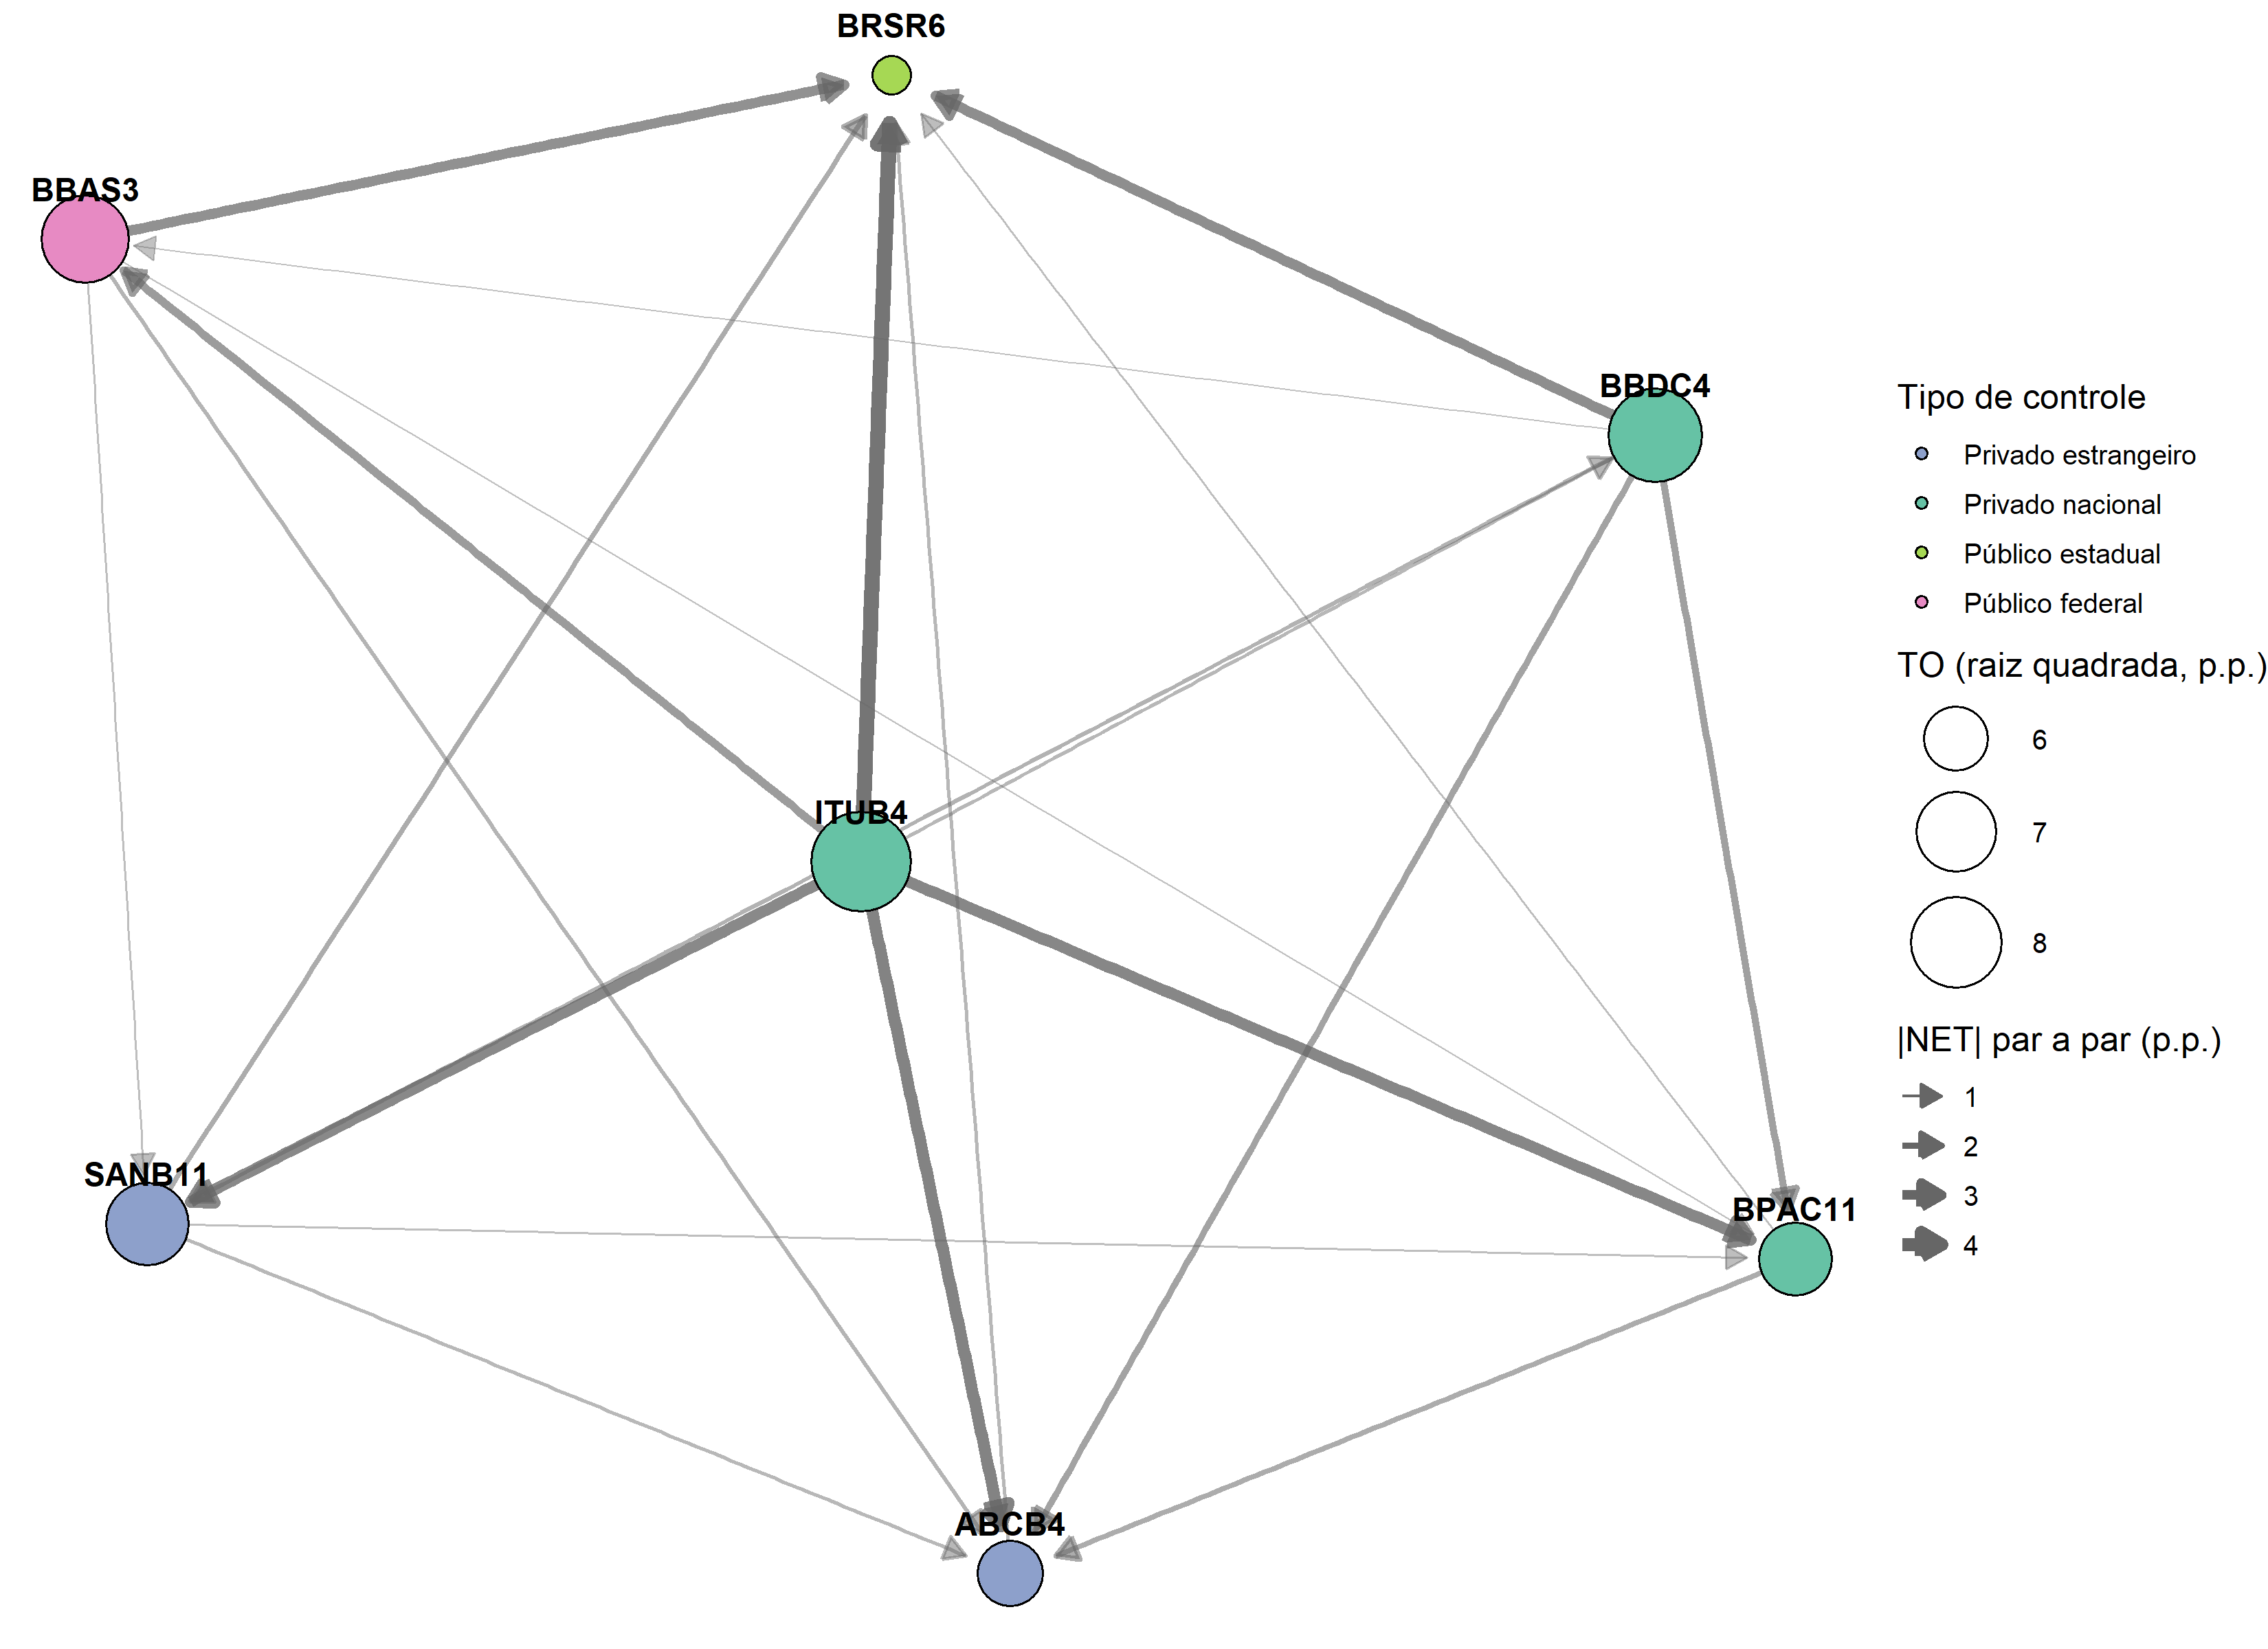
\includegraphics[width=\textwidth]{figuras/rede_n7_amostra_completa.png}
  \legend{Fonte: elaboração própria. VAR(2), $\tau=10$. Setas: do transmissor líquido ao
  receptor líquido de cada par; espessura crescente em $|\text{NET}_{ij}|$; tamanho do nó
  crescente com o TO$_i$; cor: tipo de controle. Limiar de visualização de 5\% do par mais
  forte, que retém os 21 pares. Posição dos nós: Fruchterman-Reingold.}
\end{figure}
 
\begin{figure}[H]
  \centering
  \caption{Rede líquida de conectividade, amostra completa (painel de extensão)}
  \label{fig:rede-n8}
  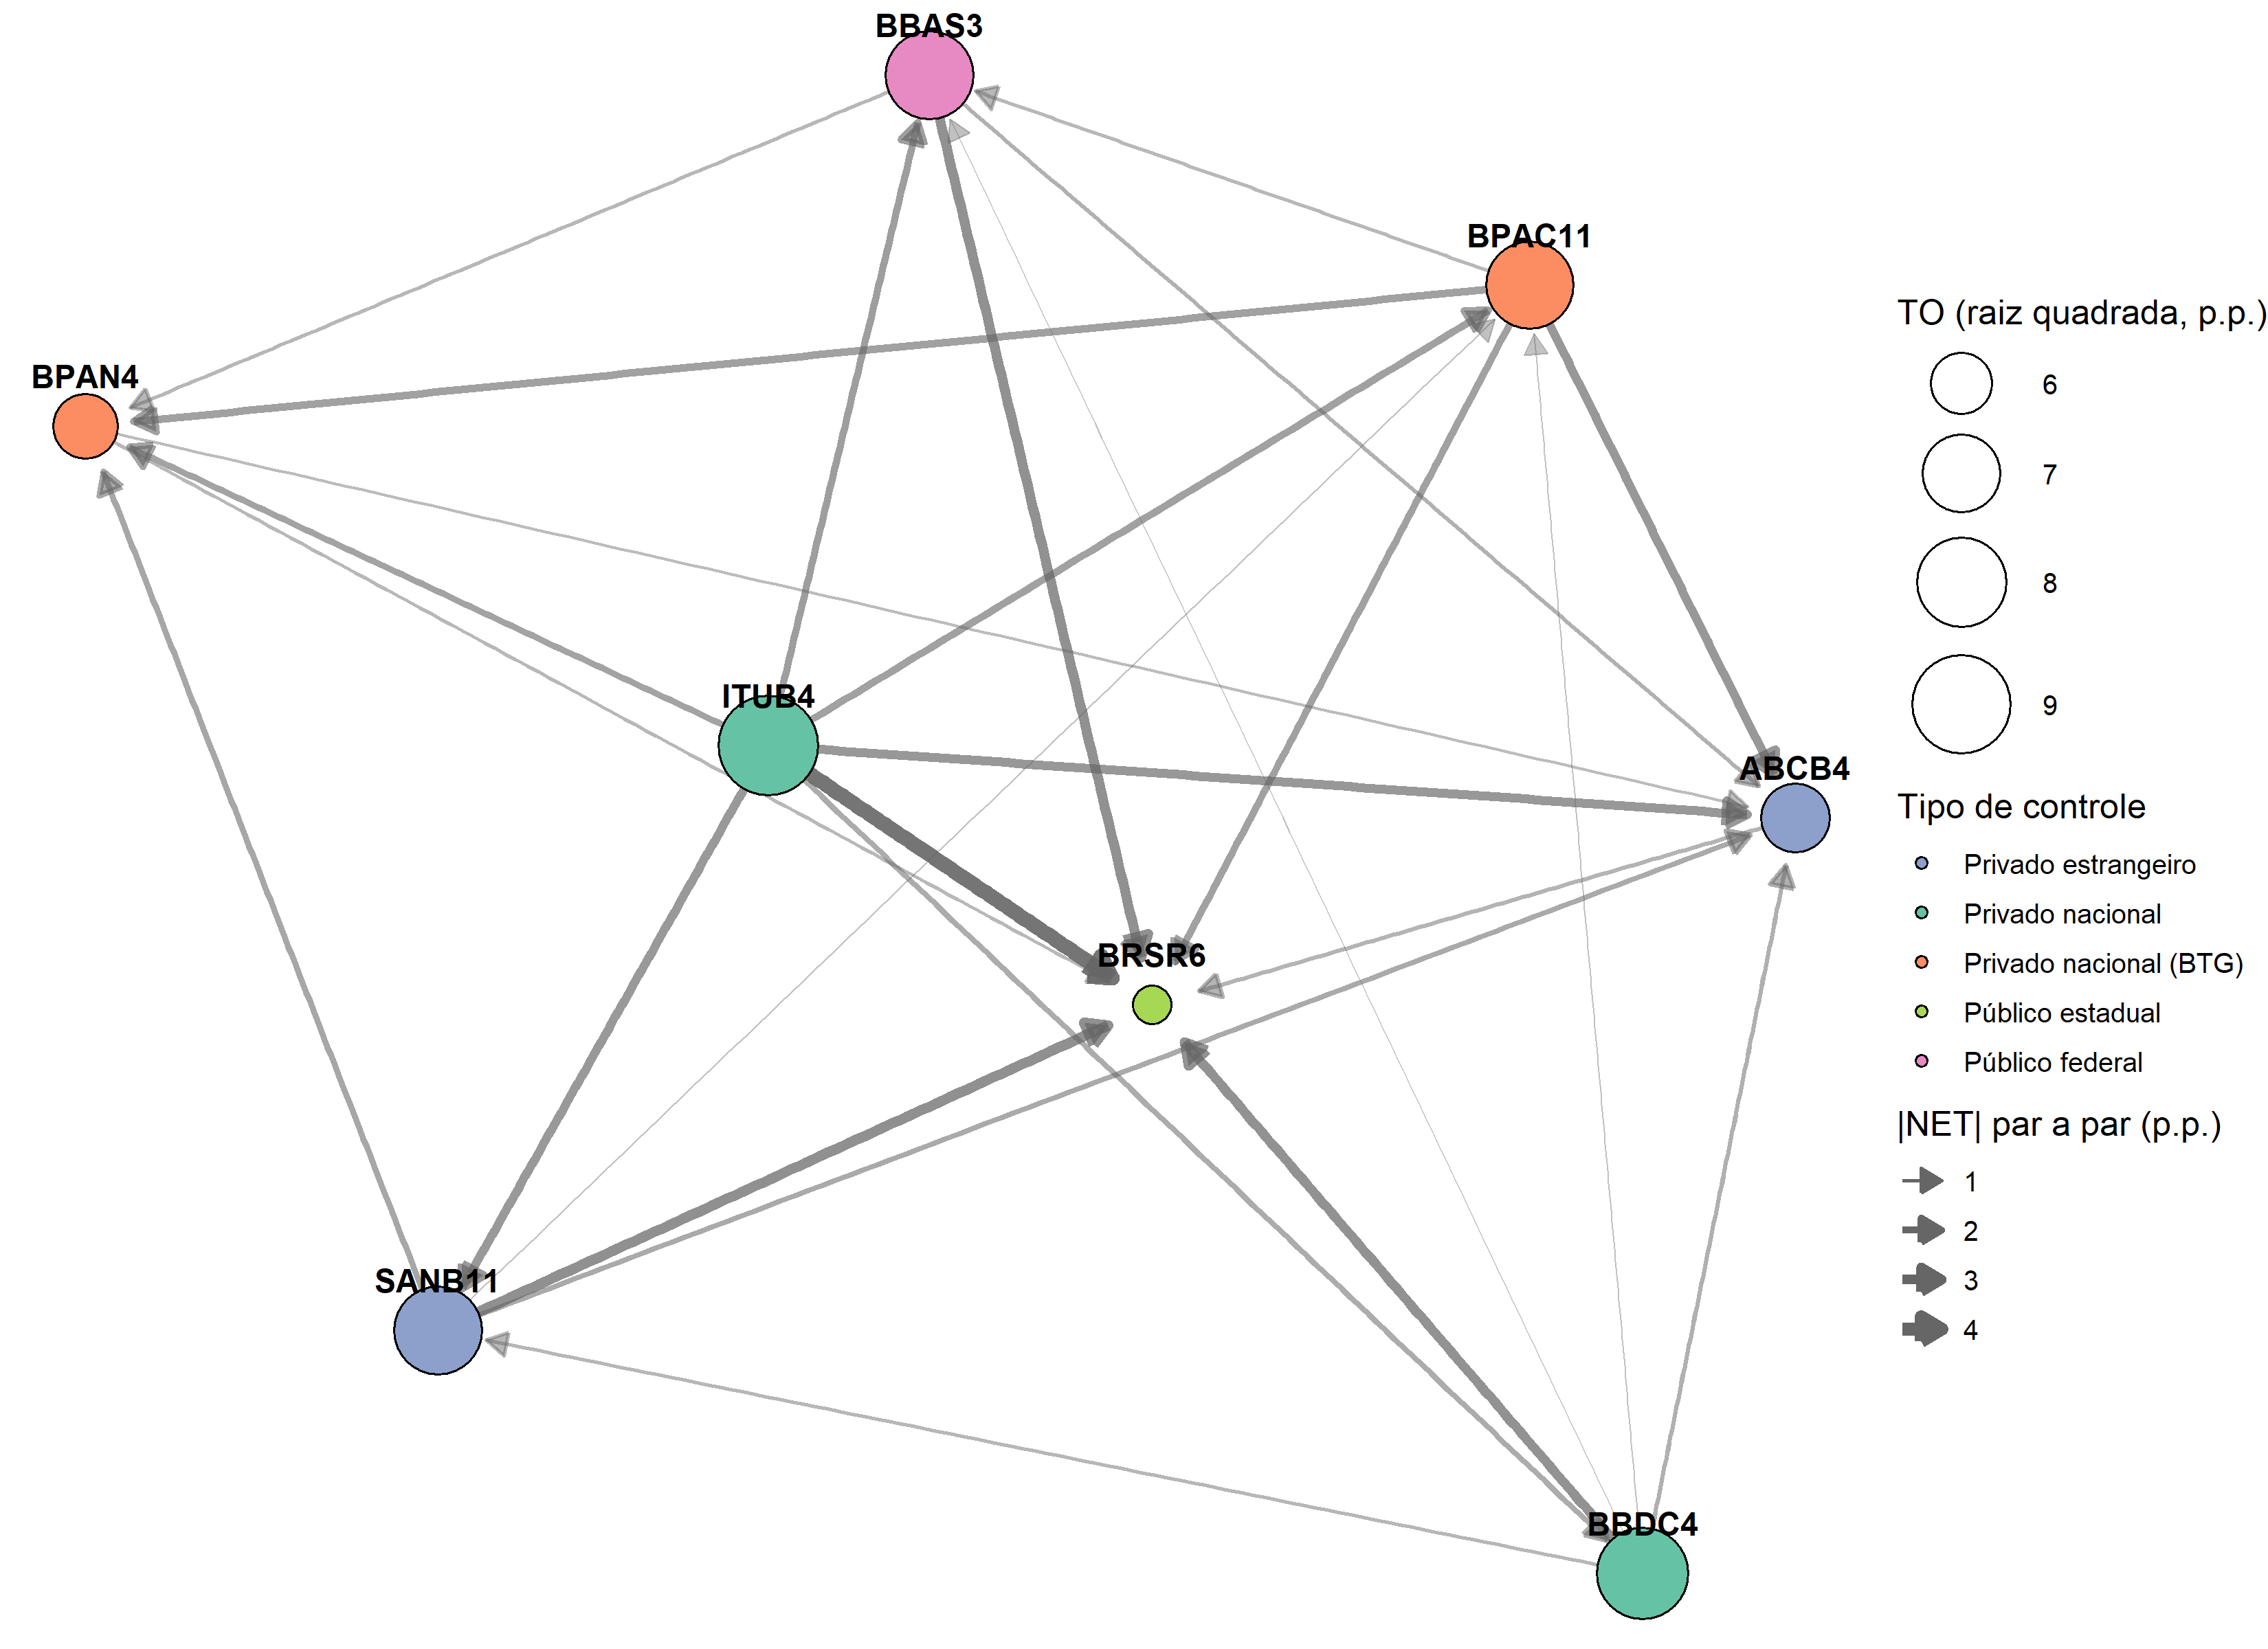
\includegraphics[width=\textwidth]{figuras/rede_n8_amostra_completa.png}
  \legend{Fonte: elaboração própria. Mesma construção da Figura~\ref{fig:rede-n7}; o limiar de
  5\% retém 26 dos 28 pares. BTG e Pan, ligados por controle societário, têm cor própria.}
\end{figure}

% ------------------------------------------------------------------------------
\section{Conectividade dinâmica}
\label{sec:res-dinamica}
% ------------------------------------------------------------------------------

A Figura~\ref{fig:tci-tvpvar} mostra o TCI do TVP-VAR do painel principal, e a
Tabela~\ref{tab:eventos} reúne os eventos do período, com data e fonte. A
série completa é exibida, mas as primeiras 200 observações, até 27/07/2018,
usadas como treino na seleção dos fatores, devem ser lidas com cautela: o
\textit{prior} usa a amostra completa, e o índice inicial (52,9\%) coincide com
o estático. Entre 2019 e fevereiro de 2020, o índice oscila em torno de 43,1\%,
com mínimo de 32,9\% em 13/02/2020. A pandemia inaugura um regime distinto: o TCI
vai de 46,0\% em 06/03/2020 para 53,1\% em 09/03, 63,8\% em 12/03 e 68,2\% em
13/03, e supera 70\% a partir de 24/03. Ele não volta a cair em seguida: de abril
de 2020 a meados de março de 2021 permanece entre 70,8\% e 74,9\% (média de
73,2\%), com máximo de 74,9\% em 16/06/2020, cerca de 30 pontos percentuais
acima do nível anterior. O declínio é gradual, com o índice abaixo de 60\% só em
10/08/2021 e abaixo de 50\% em 20/05/2022, e a mínima de 33,7\% em 20/02/2024.

Os demais episódios da Tabela~\ref{tab:eventos} são de outra ordem. O início do
aperto monetário, em 17/03/2021, não coincide com uma elevação: o TCI está em
72,1\% nessa data e desce para 60,7\% em junho. A divulgação das inconsistências
contábeis da Americanas, em 11/01/2023, é precedida por uma subida: o índice vai
de 38,1\% em 30/09/2022 a 53,0\% em 20/12/2022 e está em 50,9\% na data do fato
relevante e em 50,5\% vinte pregões depois. O anúncio do pacote fiscal, em
27/11/2024, também não produz salto: o TCI está em 47,5\% nessa data, na mesma
faixa dos 15 meses seguintes (média de 48,1\% de outubro de 2024 a dezembro de
2025), depois de ter subido de 33,7\% em fevereiro do mesmo ano.

Em 2026, o índice parte de 43,3\% em 27/02, sobe em degrau de 53,7\% para 57,5\%
em 08/04, atinge 58,7\% em 10/04 e permanece acima de 55\% até 31/07; recua para
53,2\% em agosto e 52,5\% em setembro e termina a amostra em 53,3\%. Comparam-se
três níveis: a média de 2025 (48,0\%), a de abril e maio de 2026 (56,5\%) e o
platô da pandemia (73,2\%). A elevação de 2026 sobre 2025 é de 8,5 pontos
percentuais, contra 30,1 da pandemia sobre o nível anterior (73,2\% contra
43,1\%), isto é, cerca de 28\% dela, e o pico de 2026 fica 16 pontos abaixo do de
2020. Por isso a elevação de 2026 é descrita como elevação da conectividade no
fim da amostra, e não como um regime no mesmo plano da pandemia. A causa não foi
identificada: não foi localizada fonte que registre, na data do degrau, evento
que a explique. A hipótese de elevação em períodos de instabilidade se sustenta,
assim, com clareza para a pandemia e apenas em parte para 2022--2023. A elevação
de 2026 é menor e sem causa identificada, e a hipótese não se sustenta para o
aperto da Selic nem para o pacote fiscal de 2024.

\begin{table}[H]
\centering
\caption{Cronologia de eventos do período e nível do TCI}
\label{tab:eventos}
\small
\begin{tabular}{lp{5.4cm}cp{3.2cm}}
\toprule
Data & Evento & TCI ($-20$ / 0 / $+20$) & Fonte \\
\midrule
11/03/2020 & A OMS caracteriza a COVID-19 como pandemia
  & 32,9 / 57,4 / 72,5 & \parencite{who2020} \\
17/03/2021 & O Copom eleva a Selic de 2,00\% para 2,75\% a.a., primeira alta desde 2015
  & 71,1 / 72,1 / 67,7 & \parencite{reuters2021copom} \\
11/01/2023 & A Americanas divulga inconsistências contábeis estimadas em R\$~20
  bilhões; as ações caem mais de 70\% em 12/01
  & 50,7 / 50,9 / 50,5 & \parencite{americanas2023, poder3602023} \\
27/11/2024 & O governo anuncia pacote de contenção de gastos (R\$~70 bilhões em dois
  anos) e isenção do IR até R\$~5 mil; o dólar ultrapassa R\$~6,00 pela primeira
  vez em 28/11 e fecha a R\$~5,98
  & 50,4 / 47,5 / 47,0 & \parencite{dgabc2024, sul212024} \\
13/10/2025 & O BTG Pactual divulga, à noite, fato relevante com a proposta de
  incorporação das ações do Banco Pan & -- & \parencite{btg2025} \\
09/12/2025 & Os acionistas do Pan aprovam a incorporação em assembleia
  & -- & \parencite{moneytimes2025} \\
\bottomrule
\end{tabular}
\legend{Fonte: elaboração própria. TCI do TVP-VAR do painel principal, 20 pregões
antes, na data e 20 pregões depois. A elevação de abril de 2026 não consta da
tabela porque sua causa não foi identificada.}
\end{table}

\begin{figure}[H]
  \centering
  \caption{Índice de conectividade total: TVP-VAR (painel principal)}
  \label{fig:tci-tvpvar}
  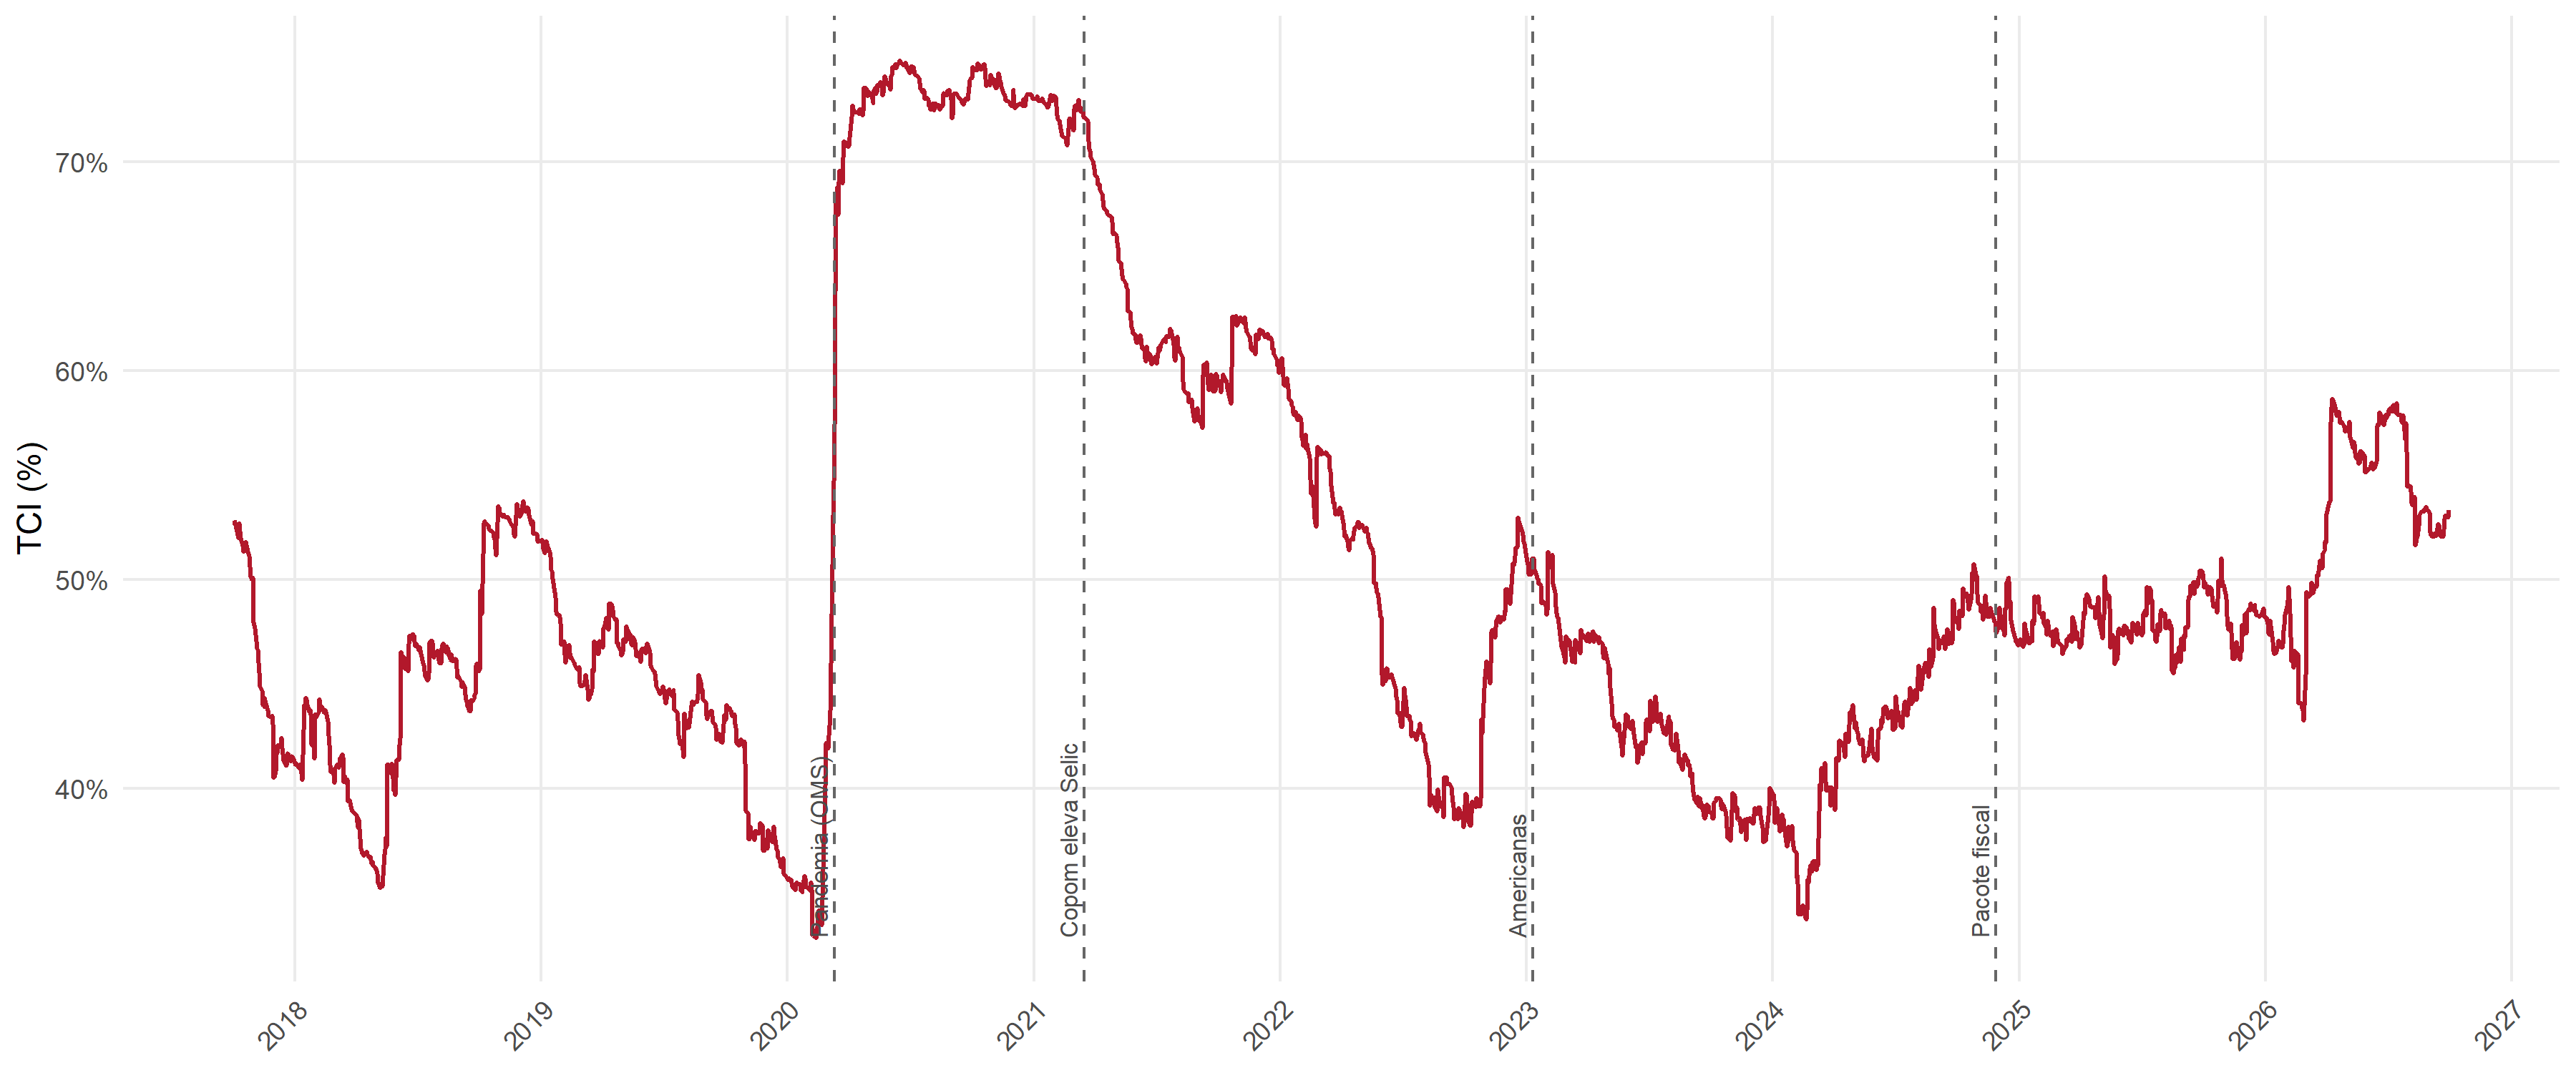
\includegraphics[width=\textwidth]{figuras/tci_tvpvar.png}
  \legend{Fonte: elaboração própria. $\kappa_1=0{,}995$, $\kappa_2=0{,}99$, $\tau=10$.
  Linhas tracejadas: eventos da Tabela~\ref{tab:eventos}.}
\end{figure}

A Figura~\ref{fig:rede-subperiodos} compara a rede líquida do painel principal em quatro
subperíodos: pré-COVID (01/08/2019 a 29/02/2020), COVID-19 (01/03 a 31/08/2020), aperto da
Selic (17/03 a 17/09/2021) e Americanas (12/01 a 12/07/2023). Cada painel reestima o VAR e a
decomposição da variância no próprio subperíodo, de 124 a 144 pregões, de modo que parte das
diferenças entre painéis é ruído de estimação. As posições dos nós são as da amostra completa,
de modo que as diferenças visuais refletem a reconfiguração das arestas e não o
reposicionamento. A figura serve para verificar se a hierarquia da amostra completa (Itaú e
Bradesco como emissores líquidos, Banrisul e ABC Brasil como receptores) se mantém em cada
subperíodo; a evidência sobre a variação do nível de conectividade é a do TVP-VAR
(Figura~\ref{fig:tci-tvpvar}). A versão do painel de extensão está no
Apêndice~\ref{ap:redes}.
 
\begin{figure}[H]
  \centering
  \caption{Rede líquida de conectividade por subperíodo (painel principal)}
  \label{fig:rede-subperiodos}
  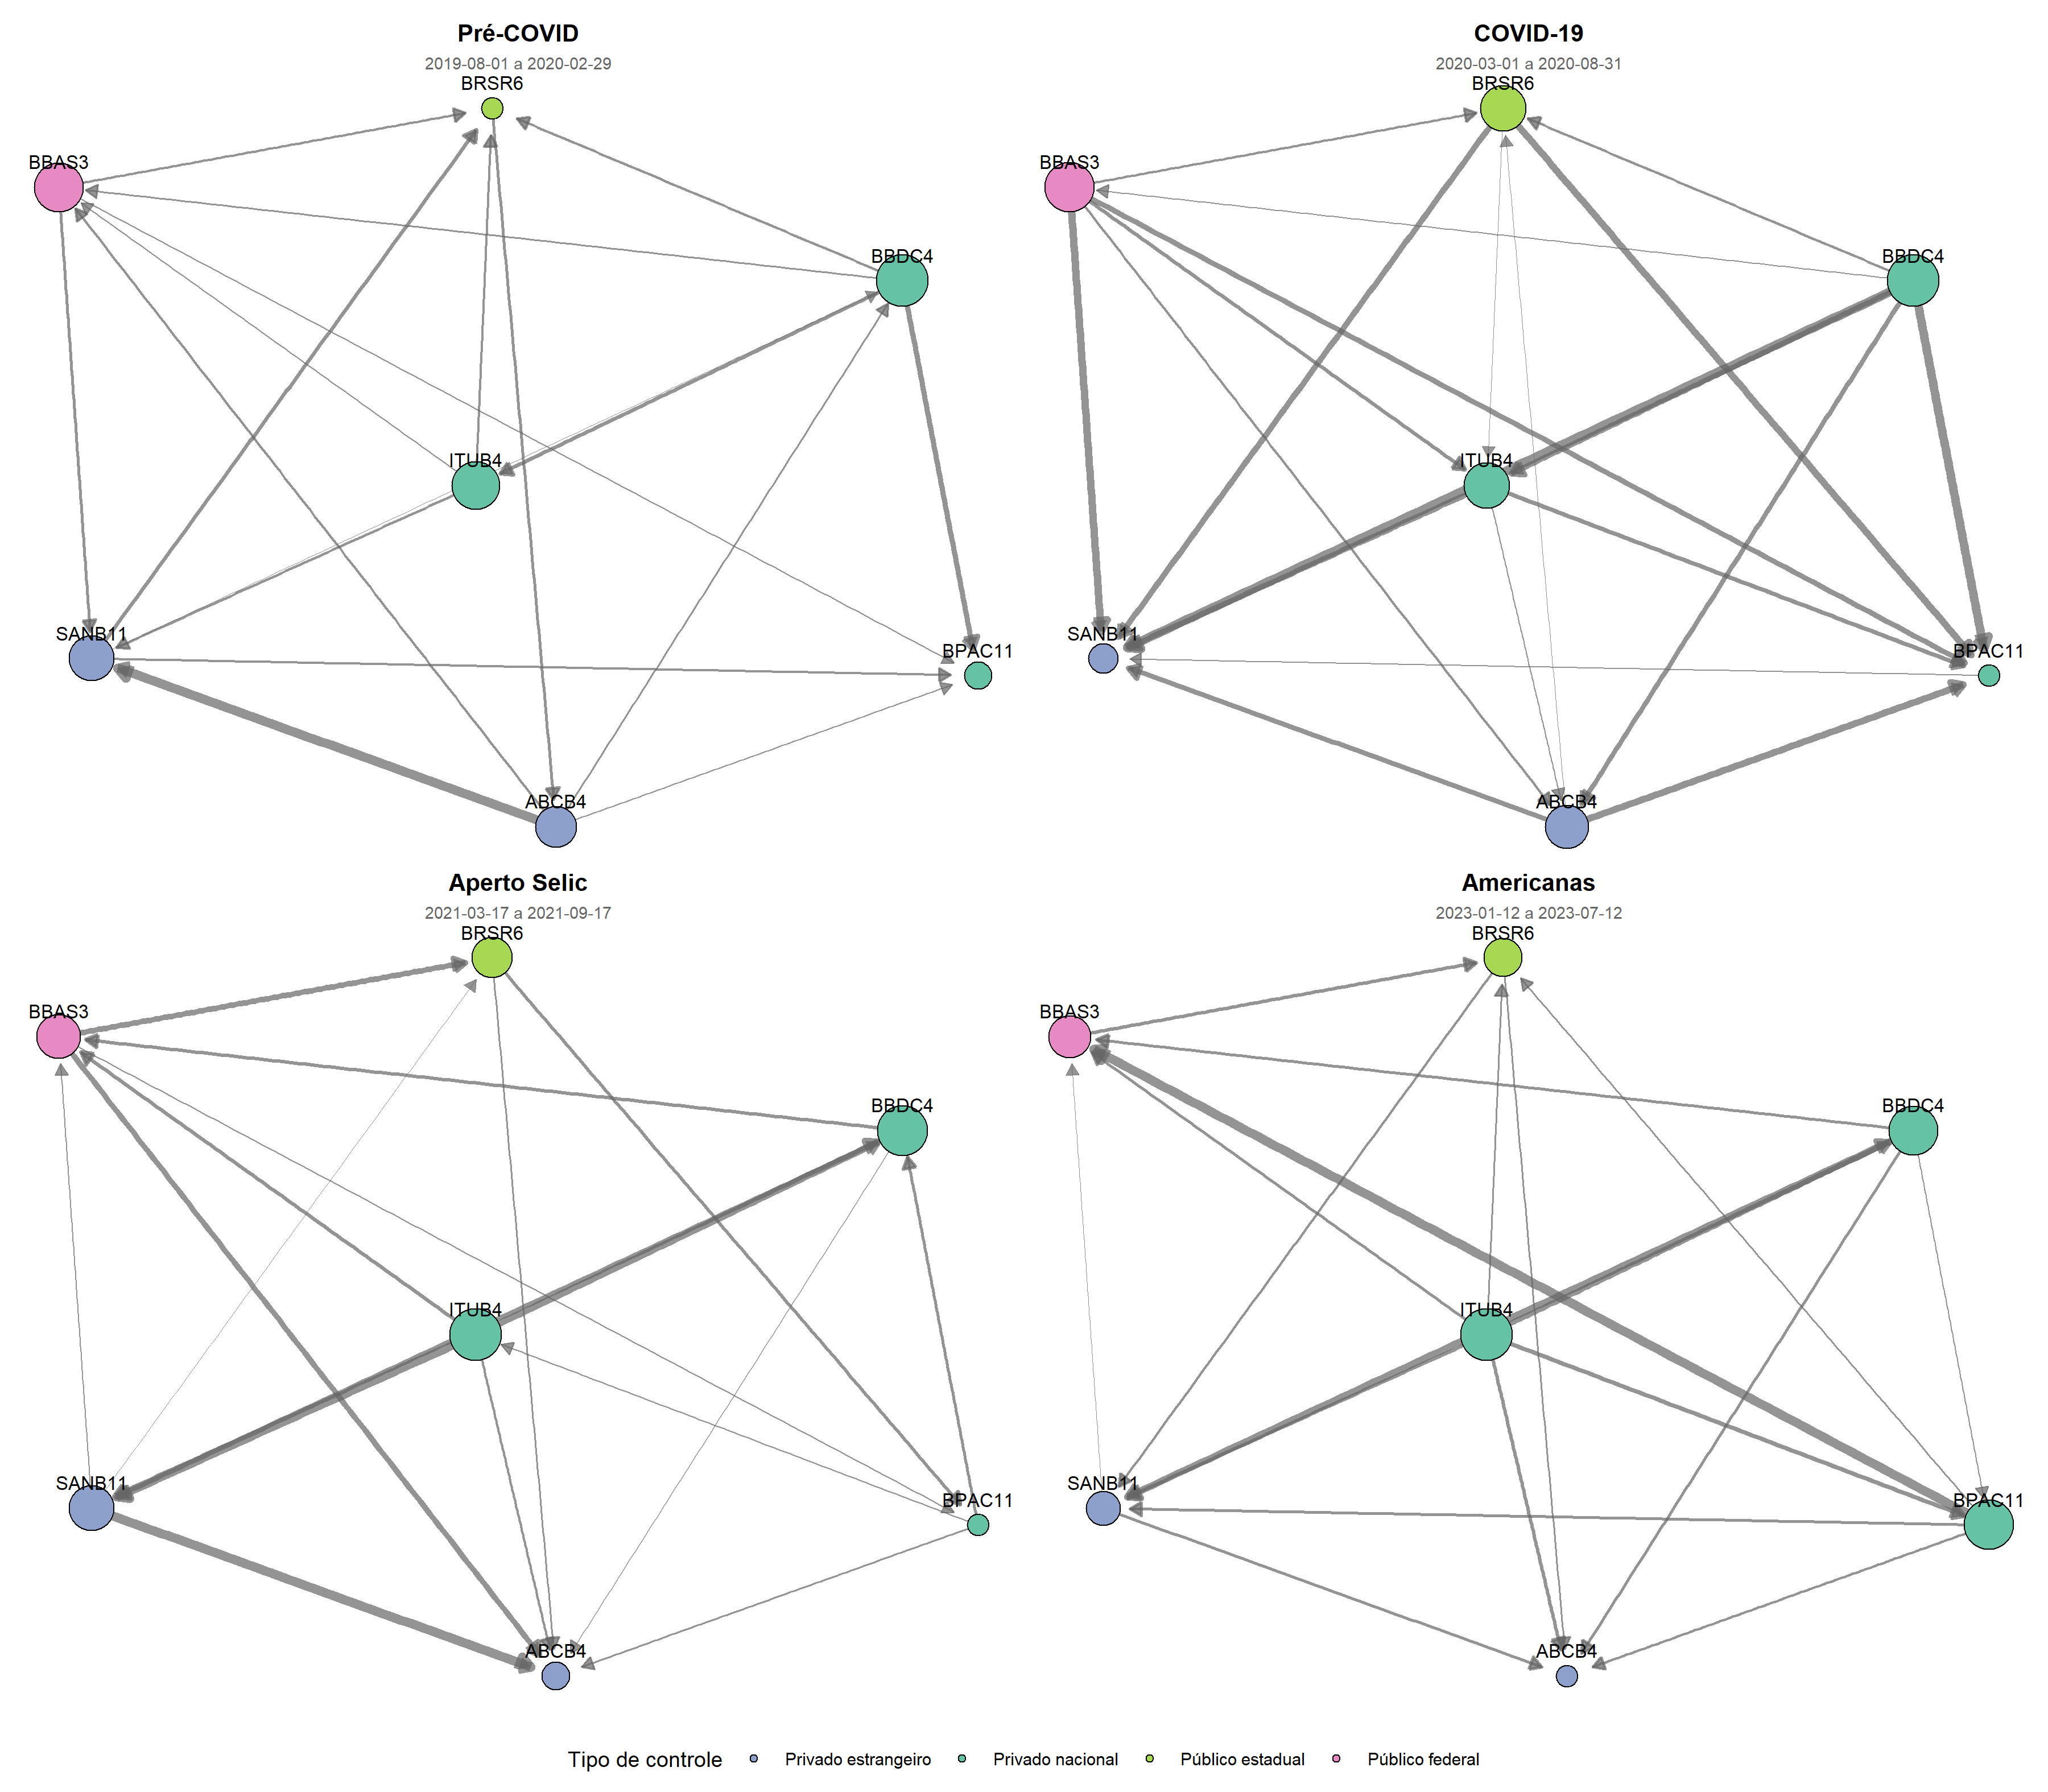
\includegraphics[width=\textwidth]{figuras/rede_n7_subperiodos.png}
  \legend{Fonte: elaboração própria. VAR(2) estático e GFEVD ($\tau=10$) estimados em cada
  subperíodo; limiar de 5\% do par mais forte de cada subperíodo. Setas, espessura, tamanho e
  cor como na Figura~\ref{fig:rede-n7}. Posições dos nós fixas, as da amostra completa.}
\end{figure}

% ------------------------------------------------------------------------------
\section{Regressão diádica}
\label{sec:res-diadica}
% ------------------------------------------------------------------------------

A Tabela~\ref{tab:diadica-agregada} apresenta a regressão da
Equação~\eqref{eq:diadica} sobre a matriz da amostra completa. No painel
principal, a indicadora de mesma natureza de controle (estatal ou privada) tem
coeficiente de 1,43 ponto percentual ($p=0{,}021$), e a de ambos de grande porte,
de 3,29 ($p=0{,}046$). No painel de extensão, os coeficientes são de 0,80
($p=0{,}041$) e 3,92 ($p=0{,}002$), e o vínculo societário BTG--Pan soma 5,92
pontos percentuais ($p<0{,}001$) além do que natureza de controle e porte
explicam. Como a amostra tem apenas dois bancos estatais, a indicadora de
natureza de controle é identificada exclusivamente pelo par Banco do Brasil e
Banrisul. A Tabela~\ref{tab:diadica-par} separa o efeito de pares específicos: o
par Itaú-Bradesco troca 6,00 (painel principal) e 5,34 (extensão) pontos
percentuais a mais de variância do que a propensão geral de cada banco prevê
($p<0{,}001$), o par Banco do Brasil-Banrisul, 2,20 ($p=0{,}029$) e 1,13
($p=0{,}075$), e o par ABC Brasil-Santander, $-1{,}33$ ($p=0{,}42$) e $-1{,}22$
($p=0{,}23$). Com os pares incluídos, o efeito de ambos de grande porte é de 2,29
($p=0{,}14$) no painel principal e de 3,10 ($p=0{,}004$) no de extensão. O
resultado de corte único tem baixa precisão, porque cada indicadora de par se
apoia em duas observações.

\begin{table}[H]
\centering
\caption{Regressão diádica, corte único: indicadoras agregadas}
\label{tab:diadica-agregada}
\small
\begin{tabular}{lcccc}
\toprule
 & \multicolumn{2}{c}{N = 7} & \multicolumn{2}{c}{N = 8} \\
Indicadora & Coef. (EP) & $p$ & Coef. (EP) & $p$ \\
\midrule
Mesma natureza de controle     & 1,43 (0,58) & 0,021 & 0,80 (0,38) & 0,041 \\
Ambos de grande porte          & 3,29 (1,57) & 0,046 & 3,92 (1,15) & 0,002 \\
Vínculo societário (BTG e Pan) & --          & --    & 5,92 (1,17) & $<0{,}001$ \\
\bottomrule
\end{tabular}
\legend{Fonte: elaboração própria. Efeitos fixos de emissor e de receptor;
erros-padrão clusterizados por par não dirigido.}
\end{table}

\begin{table}[H]
\centering
\caption{Regressão diádica, corte único: indicadoras por par específico}
\label{tab:diadica-par}
\small
\begin{tabular}{lcccc}
\toprule
 & \multicolumn{2}{c}{N = 7} & \multicolumn{2}{c}{N = 8} \\
Indicadora & Coef. (EP) & $p$ & Coef. (EP) & $p$ \\
\midrule
Itaú e Bradesco            & 6,00 (1,15) & $<0{,}001$ & 5,34 (0,85) & $<0{,}001$ \\
Banco do Brasil e Banrisul & 2,20 (0,95) & 0,029 & 1,13 (0,62) & 0,075 \\
ABC Brasil e Santander     & $-1{,}33$ (1,64) & 0,425 & $-1{,}22$ (0,99) & 0,227 \\
BTG e Pan                  & --          & --    & 5,46 (0,94) & $<0{,}001$ \\
Ambos de grande porte      & 2,29 (1,49) & 0,138 & 3,10 (1,01) & 0,004 \\
\bottomrule
\end{tabular}
\legend{Fonte: elaboração própria.}
\end{table}

A Tabela~\ref{tab:diadica-temporal} reestima a regressão ao fim de cada mês, com a
matriz do TVP-VAR (108 cortes no painel principal e 82 no de extensão). No painel
principal, o par Itaú-Bradesco tem sinal positivo em todos os cortes (média de
6,68 pontos percentuais), o par Banco do Brasil-Banrisul em 82 de 108 (média de
1,99), a indicadora de ambos de grande porte em 93 de 108 (média de 2,25), e o par
ABC Brasil-Santander é negativo em 78 de 108 (média de $-1{,}08$). No painel de
extensão, os mesmos sinais aparecem: Itaú-Bradesco e ambos de grande porte
positivos em todos os 82 cortes (médias de 5,94 e 2,94), BTG--Pan em 76 de 82
(4,89), Banco do Brasil-Banrisul em 52 de 82 (1,27) e ABC Brasil-Santander
negativo em 61 de 82 ($-0{,}87$). Os coeficientes de meses vizinhos são quase iguais, porque o TVP-VAR é suave. O teste
$t$ da média, que trata os cortes como independentes, superestima a evidência e é
reportado apenas como referência. A evidência principal é a proporção de cortes com
o mesmo sinal.

\begin{table}[H]
\centering
\caption{Regressão diádica por par específico: cortes mensais do TVP-VAR}
\label{tab:diadica-temporal}
\small
\begin{tabular}{lccc}
\toprule
Indicadora & Média & Positivos & $t$ \\
\midrule
\multicolumn{4}{l}{\textit{Painel principal (N = 7), 108 cortes}} \\
Itaú e Bradesco            & 6,68 & 108/108 & 19,95 \\
Banco do Brasil e Banrisul & 1,99 &  82/108 &  8,74 \\
ABC Brasil e Santander     & $-1{,}08$ & 30/108 & $-5{,}43$ \\
Ambos de grande porte      & 2,25 &  93/108 & 10,32 \\
\midrule
\multicolumn{4}{l}{\textit{Painel de extensão (N = 8), 82 cortes}} \\
Itaú e Bradesco            & 5,94 &  82/82 & 19,62 \\
BTG e Pan                  & 4,89 &  76/82 & 12,77 \\
Banco do Brasil e Banrisul & 1,27 &  52/82 &  5,27 \\
ABC Brasil e Santander     & $-0{,}87$ & 21/82 & $-4{,}30$ \\
Ambos de grande porte      & 2,94 &  82/82 & 22,32 \\
\bottomrule
\end{tabular}
\legend{Fonte: elaboração própria. $t$ da média dos coeficientes mensais contra zero,
sem correção de autocorrelação.}
\end{table}

Três padrões se repetem nos dois painéis. Primeiro, os dois maiores bancos
privados trocam mais risco entre si do que o porte e a propensão geral de cada um
explicam, sem que haja vínculo de controle entre eles. O mecanismo compatível é a
proximidade de modelo de negócio e de exposição a choques comuns. Segundo, os dois
bancos estatais também têm coeficiente positivo, em magnitude menor e com
evidência mais frágil no painel de extensão ($p=0{,}075$ no corte único e 52 de 82
cortes positivos). Terceiro, o par classificado sob a etiqueta nominal de privado
estrangeiro, ABC Brasil e Santander, não apresenta conectividade adicional, sendo o
coeficiente negativo na média e na maior parte dos cortes, mas não se distingue
de zero no corte único. Compartilhar um rótulo de classificação não produz, por si só,
comovimento. O vínculo BTG--Pan é tratado na Seção~\ref{sec:btg-pan}.

% ------------------------------------------------------------------------------
\section{O vínculo societário BTG--Pan}
\label{sec:btg-pan}
% ------------------------------------------------------------------------------

A hipótese de que o vínculo de controle societário produz comovimento de
volatilidade além do que a propensão geral de cada banco prevê não pode ser
testada no painel principal, pela razão evidente de que nele não há nenhum par de
instituições ligadas por controle. Recorre-se, por isso, ao painel de extensão,
único em que o par BTG Pactual e Banco Pan está presente. A restrição não decorre
de escolha metodológica, e sim do fato de que, no sistema bancário brasileiro
listado, esse é o único vínculo dessa natureza disponível no período.

No corte único (Tabela~\ref{tab:diadica-par}), o par BTG--Pan tem o maior
coeficiente da tabela, 5,46 pontos percentuais ($p<0{,}001$), seguido de perto
pelo par Itaú-Bradesco (5,34). Na especificação agregada
(Tabela~\ref{tab:diadica-agregada}), a indicadora de vínculo soma 5,92 pontos
percentuais além do que a natureza de controle e o porte explicam. O par
classificado apenas sob a etiqueta nominal de privado estrangeiro, ABC Brasil e
Santander, duas instituições sem proximidade de porte ou de modelo de negócio, não
se distingue de zero ($-1{,}22$; $p=0{,}23$). A leitura não se resume, porém, a
vínculo societário organiza a rede e categoria nominal não. O par Itaú-Bradesco,
os dois maiores bancos privados nacionais e sem vínculo de controle entre si,
também tem coeficiente elevado, e a diferença para o do par BTG--Pan, de 0,12
ponto percentual, é pequena frente aos erros-padrão (0,94 e 0,85). Como a regressão
já controla pelo efeito de ambos serem instituições de grande porte (3,10 ponto
percentual, $p=0{,}004$), o coeficiente de Itaú-Bradesco representa um comovimento
adicional, específico do par, que não é explicado nem pela propensão geral de cada
banco a transmitir e receber risco, nem pelo porte. Duas explicações são
compatíveis com os dados: o vínculo de controle societário, no caso do par
BTG--Pan, e a proximidade de modelo de negócio e de exposição a choques
regulatórios e macroeconômicos comuns aos dois maiores bancos de varejo do país,
no caso do par Itaú-Bradesco, mecanismos distintos mas igualmente capazes de gerar
comovimento além do que porte e propensão geral já explicam. Os dados não permitem
distinguir entre as duas hipóteses para o par Itaú-Bradesco, na ausência de um
vínculo de controle a testar. O achado central permanece. O controle societário é
suficiente para gerar comovimento da mesma ordem de grandeza que a maior
proximidade de porte e de modelo de negócio da amostra, mas não é o único
mecanismo capaz de fazê-lo.

A robustez do resultado não depende de um único corte (Tabela~\ref{tab:diadica-temporal}).
O coeficiente do par BTG--Pan é positivo em 76 dos 82 cortes mensais (93\%), com
média de 4,89 pontos percentuais ($t$ de 12,77). Os seis
cortes negativos estão entre agosto de 2023 e abril de 2025 (agosto e setembro de
2023, março de 2024 e fevereiro a abril de 2025).

A Figura~\ref{fig:coef-btgpan-tempo} e as Tabelas~\ref{tab:btgpan-anual} e~\ref{tab:btgpan-regime}
mostram a evolução do coeficiente. O BTG Pactual assumiu o controle pleno do Banco Pan em maio de
2021, ao adquirir a totalidade da participação até então detida pela Caixa Econômica Federal e
encerrar o controle compartilhado que mantinha desde 2011
\footnote{BANCO PAN. \textit{Nossa História}. Relações com Investidores,
2021. Disponível em:
\url{https://ri.bancopan.com.br/show.aspx?idCanal=98FuehC2XKrWRMgsqA5Tpw==&linguagem=pt}.
Acesso em: 21/09/2026.}.
Em junho de 2020, o BTG já detinha 41,52\% do capital total do Pan (50,81\% das ordinárias e 30,35\%
das preferenciais), sem mudança no controle nem no acordo de acionistas \parencite{pan2020comunicado}.
Sob controle compartilhado (janeiro de 2019 a abril de 2021), o coeficiente é positivo nos 28
cortes, com média de 6,31 pontos percentuais. Sob controle integral (maio de 2021 a outubro de
2025), a média é de 4,14, mas a série se divide em dois períodos: de maio de 2021 a dezembro de
2022, a média é de 8,52, com máximo de 13,65 em 30/06/2022; de janeiro de 2023 a outubro de 2025,
é de 1,57, e os seis cortes negativos da amostra, todos nesse período, ficam entre agosto de 2023
e abril de 2025. O comovimento específico do par é, assim, menor de 2023 em diante, justamente
quando o BTG tem o controle integral há mais tempo, o oposto do que o mecanismo proposto sugeriria,
e é maior em 2021--2022 sob o mesmo controle. A trajetória não segue, portanto, a cronologia do
controle. O resultado de média, que é robusto (coeficiente positivo em 76 dos 82 cortes), sustenta
a conclusão da seção mas a variação no tempo fica como achado em aberto, e nenhuma explicação para
ela é proposta aqui, porque não foi testada. Dentro de 2025, o coeficiente vai de $-1{,}07$ em 31/03
a 3,27 no último corte, em 13/10/2025. Como a amostra termina nesse pregão, antes de o BTG divulgar,
na noite do mesmo dia, o fato relevante da proposta de incorporação \parencite{btg2025}, o painel
não permite observar o que ocorre depois.

\begin{table}[H]
\centering
\caption{Coeficiente BTG--Pan: média anual dos cortes mensais}
\label{tab:btgpan-anual}
\begin{tabular}{lcc}
\toprule
Ano & Coeficiente médio (p.p.) & Cortes \\
\midrule
2019 & 6,98 & 12 \\
2020 & 5,45 & 12 \\
2021 & 6,94 & 12 \\
2022 & 9,57 & 12 \\
2023 & 2,06 & 12 \\
2024 & 1,50 & 12 \\
2025 & 1,07 & 10 \\
\bottomrule
\end{tabular}
\legend{Fonte: elaboração própria. A média de 2019 inclui nove cortes do período
de treino do filtro.}
\end{table}

\begin{table}[H]
\centering
\caption{Coeficiente BTG--Pan por regime de controle do BTG sobre o Pan}
\label{tab:btgpan-regime}
\small
\begin{tabular}{p{6.4cm}cccc}
\toprule
Período & Cortes & Média (p.p.) & Mínimo & Positivos \\
\midrule
Controle compartilhado (jan/2019 a abr/2021) & 28 & 6,31 & 3,42 & 28/28 \\
Controle integral (mai/2021 a out/2025)      & 54 & 4,14 & $-1{,}07$ & 48/54 \\
\quad mai/2021 a dez/2022                    & 20 & 8,52 & 5,01 & 20/20 \\
\quad jan/2023 a out/2025                    & 34 & 1,57 & $-1{,}07$ & 28/34 \\
\bottomrule
\end{tabular}
\legend{Fonte: elaboração própria. O controle integral começa em maio de 2021, com a compra da
participação da Caixa. Os 28 cortes do primeiro período incluem os nove do período de treino do
filtro, sem eles, a média é de 6,20 (19 cortes).}
\end{table}

\begin{figure}[H]
  \centering
  \caption{Coeficiente da regressão diádica: BTG--Pan}
  \label{fig:coef-btgpan-tempo}
  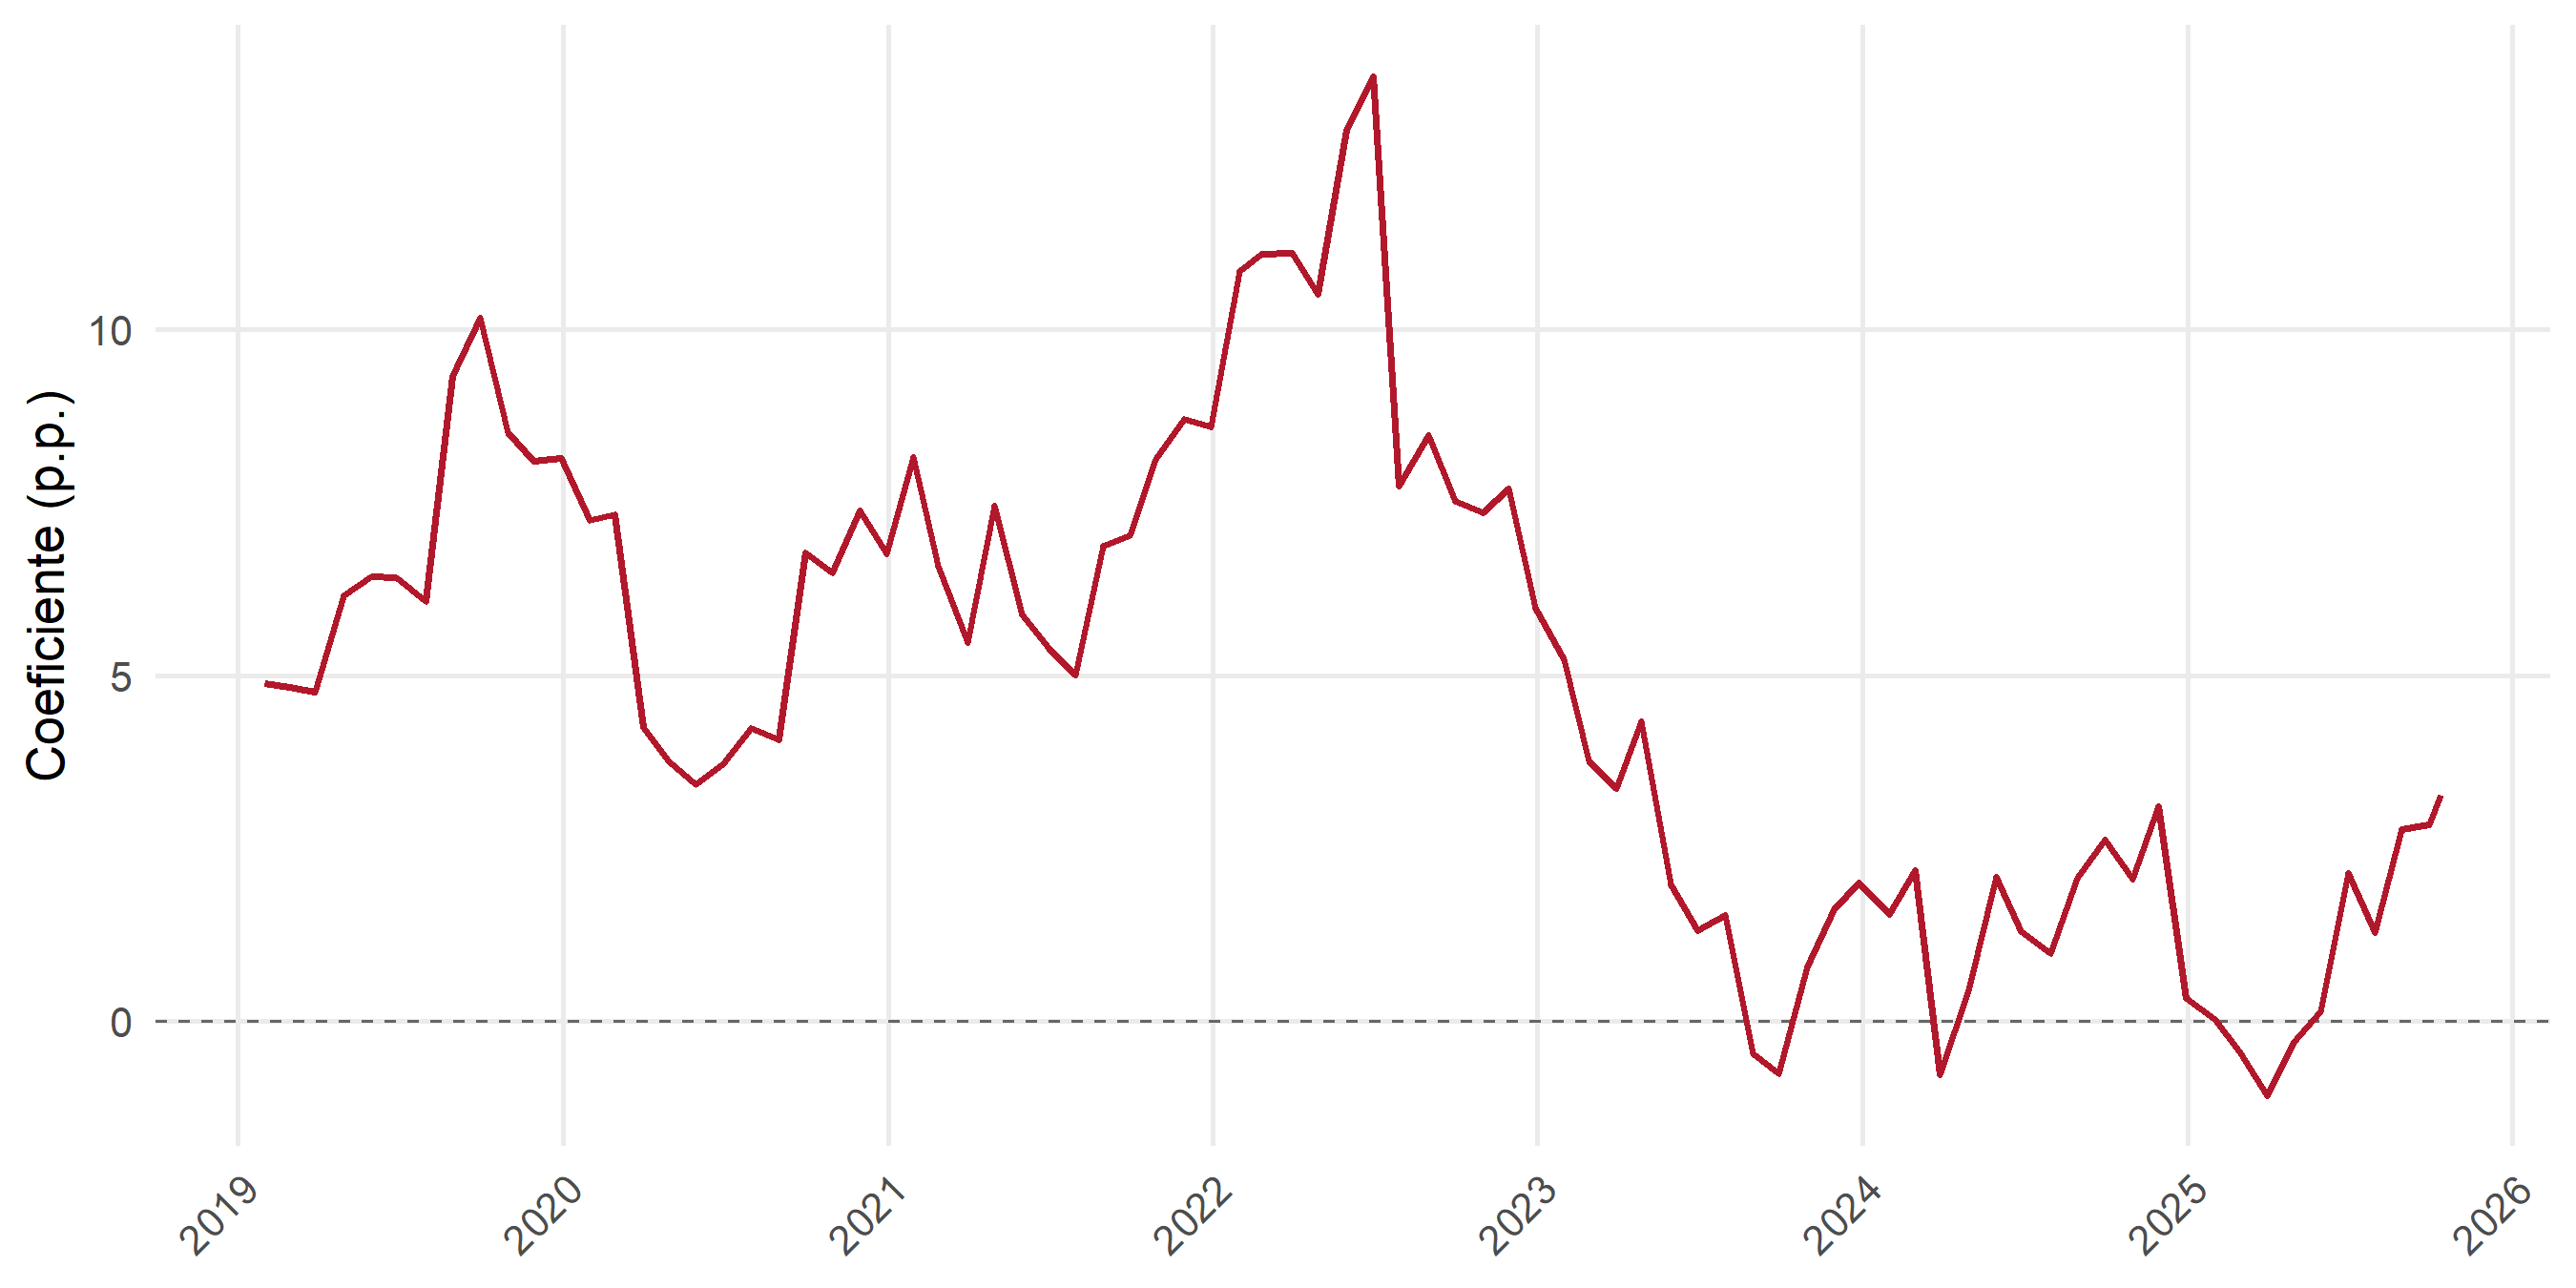
\includegraphics[width=\textwidth]{figuras/coef_btgpan_temporal.png}
  \legend{Fonte: elaboração própria. Coeficiente por corte mensal, com efeitos
  fixos de emissor e de receptor.}
\end{figure}

O desfecho de outubro de 2025 traz uma evidência adicional, de outra natureza. O fato
relevante do BTG com a proposta de incorporação é de 13/10/2025, à noite
\parencite{btg2025}. No pregão seguinte, 14/10, o Pan sobe 26,5\% (retorno logarítmico de
23,5\%) e o BTG cai 1,9\%, e a razão entre os preços de fechamento de BPAN4 e BPAC11 passa de
0,163 para 0,210, a 1,4\% da relação de troca de 0,2128 \textit{unit} do BTG por ação preferencial
do Pan. Daí até 23/01/2026, a razão fica, em média, a 0,05\% dessa relação e a menos de 2\% dela em
68 dos 69 pregões. O mercado tratou, portanto, a operação como certa desde o primeiro pregão
posterior à divulgação.

A correlação dos retornos diários confirma o diagnóstico. Ela é de 0,39 nos 69 pregões anteriores
ao anúncio e de 0,43 nos 69 posteriores, mas de 0,97 quando se exclui o dia 14/10, em que o salto do
Pan não tem contrapartida no BTG, nos nove pregões entre 15/10 e 27/10, é de 0,95. A correlação móvel
de 10 pregões reflete esse dia, e não um evento posterior: é negativa (entre $-0{,}28$ e $-0{,}11$)
enquanto o dia 14/10 está na janela e salta de $-0{,}25$ em 27/10 para 0,94 em 28/10, dia em que ele a
deixa. A série de 30 pregões da Figura~\ref{fig:corr-btgpan} tem o mesmo comportamento, com o salto em
26/11. As datas de 28/10 e 26/11 são, portanto, artefatos da janela móvel, o mesmo efeito que desloca o
pico da pandemia no Apêndice~\ref{ap:janela}. Nos últimos 10, 20, 30, 40, 50 e 60 pregões disponíveis
(até 23/01/2026, perto da deslistagem), a correlação é de 0,96, 0,95, 0,97, 0,98, 0,98 e 0,97.

\begin{figure}[H]
  \centering
  \caption{Correlação móvel de retornos: BPAN4 e BPAC11}
  \label{fig:corr-btgpan}
  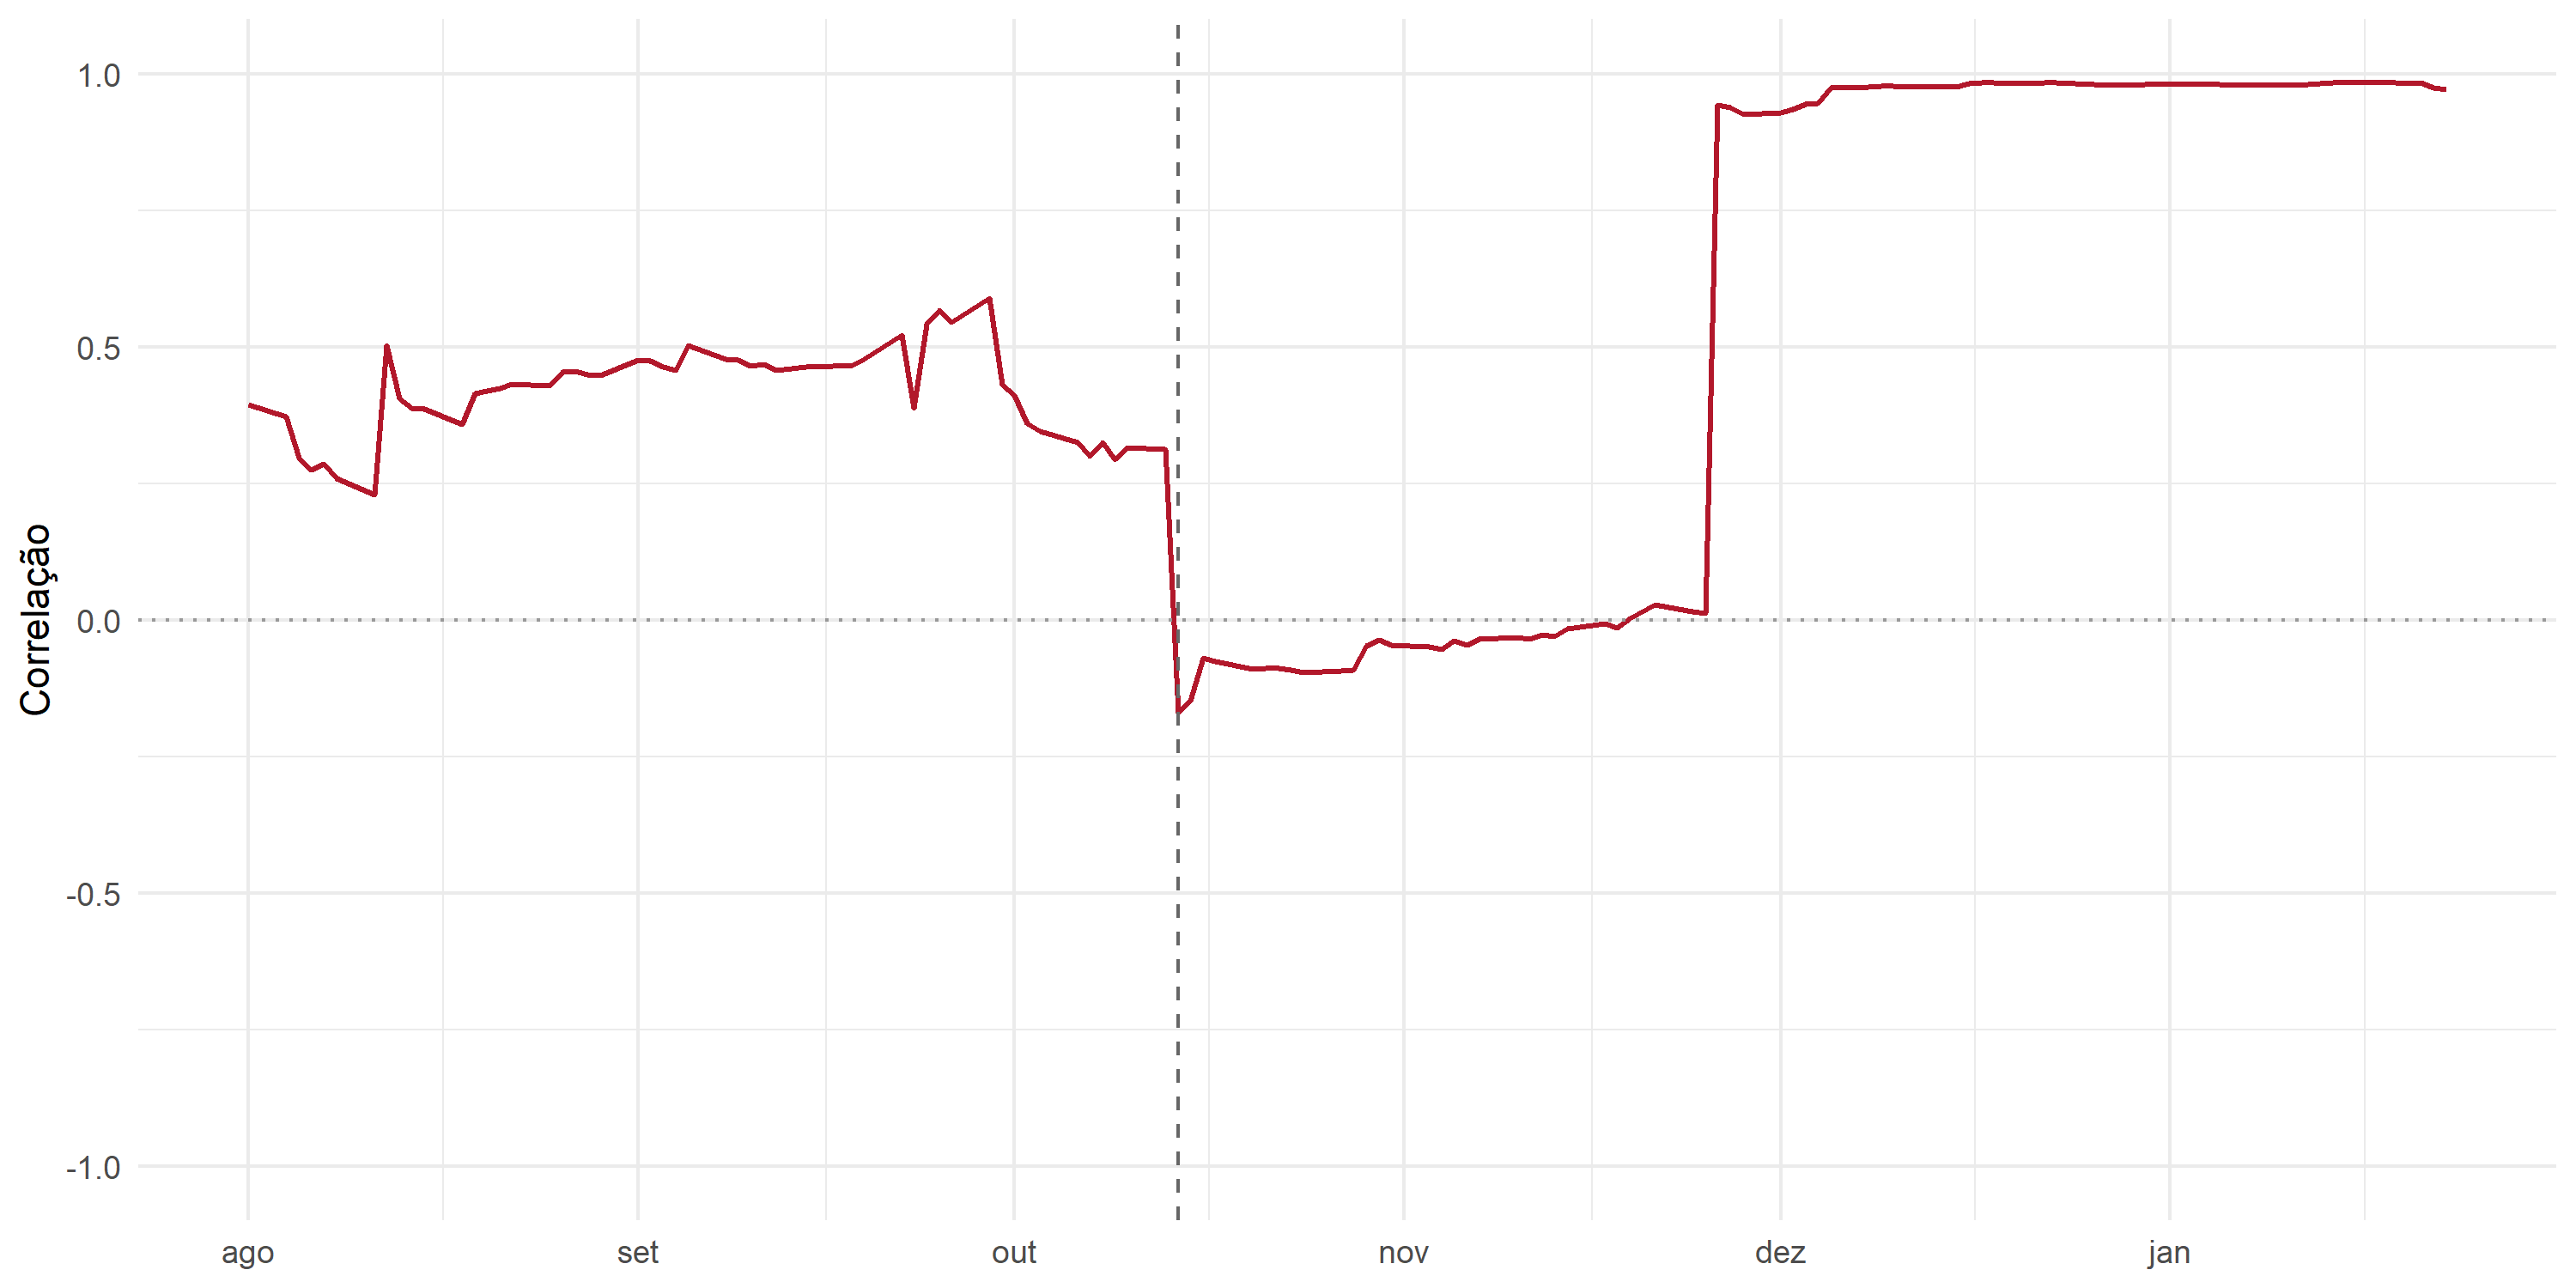
\includegraphics[width=\textwidth]{figuras/corr_bpan4_bpac11_rolling.png}
  \legend{Fonte: elaboração própria. Janela de 30 dias. Linha tracejada: 14/10/2025,
  primeiro pregão após o fato relevante de 13/10/2025. O salto de 26/11 é o dia em que o
  pregão de 14/10 deixa a janela.}
\end{figure}

A operação cumpre dois papéis na seção. Primeiro, explica por que o painel de extensão se
encerra em 13/10/2025. Desde o primeiro pregão posterior à proposta, o preço do Pan fica preso à
relação de troca e a correlação com o BTG passa a 0,97, de modo que as duas séries deixam de ser
distinguíveis para fins de decomposição de variância, e a decomposição entre elas deixaria de ser
informativa se estendida além desse ponto. Segundo, a convergência é compatível com a arbitragem sob
relação de troca fixa, que decorre dos termos da operação anunciada. Ela mostra que o mercado tratou a
fusão como certa desde o primeiro pregão, mas não distingue o efeito do vínculo de controle do efeito
dessa arbitragem e não resolve a variação do coeficiente ao longo do tempo, que permanece em aberto.

O resultado desta seção não é levado ao painel principal de sete instituições
porque o vínculo societário se encerrou no mundo real com a incorporação. Em
contrapartida, é o painel principal que permite alcançar a elevação da conectividade de
2026, fora do alcance do painel de extensão.

% ------------------------------------------------------------------------------
\section{Considerações finais}
\label{sec:consideracoes}
% ------------------------------------------------------------------------------

Este trabalho mediu a rede de spillovers de volatilidade entre os principais
bancos brasileiros listados, em sete instituições de 2017 a 2026 (painel
principal) e em oito de 2019 a outubro de 2025 (painel de extensão), a partir de um
estimador de volatilidade de um dia (Rogers-Satchell com termo \textit{overnight}),
do VAR com decomposição generalizada da variância e de um TVP-VAR com fatores de
esquecimento selecionados por verossimilhança preditiva.

A conectividade é alta e varia ao longo do tempo. O TCI estático é de 52,9\% no
painel principal e de 55,7\% no de extensão. No TVP-VAR, o índice passa de uma média
de 43,1\% antes da pandemia para um patamar de cerca de 73\% que se mantém de abril
de 2020 a março de 2021, desce gradualmente até 33,7\% em fevereiro de 2024 e volta a
subir em 2026, em uma elevação de 8,5 pontos percentuais sobre a média de 2025 (até
58,7\% em abril), cerca de 28\% da elevação da pandemia e sem causa identificada. A
hipótese de elevação em períodos de instabilidade se sustenta com clareza para a
pandemia e apenas em parte para 2022--2023, mas não para o aperto da Selic nem para
o pacote fiscal de 2024. A janela rolante data o pico da pandemia
entre 30/09/2020 e 08/02/2021, conforme a largura da janela, contra 16/06/2020 no
TVP-VAR, o que justifica a escolha do segundo.

A estrutura é heterogênea. O ranking de transmissão (TO) coloca os cinco bancos do
S1 nas cinco primeiras posições nos dois painéis. O Itaú é o maior transmissor
líquido em todas as 13 especificações de robustez de cada painel, e o Banrisul, o
maior receptor líquido na maioria delas. No painel principal, Santander e BTG, do S1,
são receptores líquidos, o que mostra que o S1, definido por porte e atividade
internacional, aproxima o ranking de transmissão, mas não o reproduz. A regressão
diádica mostra que o par Itaú-Bradesco troca mais risco do que o porte e a propensão
de cada banco explicam, que o par Banco do Brasil-Banrisul também o faz, em menor
magnitude, e que a etiqueta nominal de controle estrangeiro não produz conectividade
adicional. No painel de extensão, o par BTG--Pan, ligado por controle societário, tem
coeficiente positivo em 76 dos 82 cortes mensais e magnitude semelhante à do par
Itaú-Bradesco. A trajetória do coeficiente, porém, não segue a cronologia do controle: é menor
de 2023 em diante, sob controle integral, do que sob controle compartilhado, e permanece sem
explicação testada. A convergência dos dois papéis ao fim do processo de incorporação é
compatível com a arbitragem sob relação de troca fixa.

Os resultados têm limites. O nível do TCI depende do número de instituições (17,6\%,
37,8\%, 48,6\% e 52,9\% com 2, 4, 6 e 7 bancos) e por isso não é comparado ao de outros
estudos nem entre os painéis. As métricas de centralidade recursiva ordenam os bancos
como o FROM e não acrescentam informação nesta amostra. O \textit{prior} do TVP-VAR
final usa a amostra completa, e a seleção dos fatores usa os 200 primeiros pregões
como treino. A indicadora de mesma
natureza de controle é identificada apenas pelo par Banco do Brasil-Banrisul. O VAR
em níveis é uma aproximação de memória curta a séries de memória longa ($\hat{d}$
entre 0,47 e 0,68). Os resultados descrevem associações, não causas: a elevação de 2026 não tem
causa identificada, e a trajetória do coeficiente BTG--Pan não é explicada pela
cronologia do controle.

Duas extensões seguem naturalmente. A primeira é ampliar a amostra, com mais
instituições e dados não públicos, para testar se a heterogeneidade por controle e
por porte se mantém quando há mais pares do mesmo tipo e mais de um vínculo
societário. A segunda é estimar o modelo no domínio da frequência e nos quantis,
extensões da literatura descartadas aqui por exigirem amostras e horizontes maiores,
para verificar se a transmissão nas caudas segue a mesma hierarquia.

% ==============================================================================
% APÊNDICES
% ==============================================================================

\appendix

\chapter{Janela rolante}
\label{ap:janela}

A Figura~\ref{fig:janelas} compara o TCI do painel principal estimado por janela
rolante com $W=150$, 200 e 250. O pico do período da pandemia é datado em
30/09/2020 (77,9\%), 16/10/2020 (76,8\%) e 08/02/2021 (75,8\%), respectivamente, ou
seja, desloca-se 131 dias com a largura da janela, enquanto o do TVP-VAR é de
16/06/2020. O índice cai de 6,3 a 6,9 pontos percentuais nos 20 pregões em torno
das datas em que o colapso de março sai de cada janela (27/10/2020, 12/01/2021 e
26/03/2021), e passa a menos de 60\% em 06/01/2021, 22/03/2021 e 12/05/2021, contra
10/08/2021 no TVP-VAR. O nível e a dispersão são parecidos (TCI médio de 44,1\%,
44,0\% e 44,2\%; desvio-padrão de 12,9 a 13,7), e as séries são correlacionadas
(0,95 entre 150 e 200, 0,90 entre 150 e 250 e 0,96 entre 200 e 250), mas o degrau
acompanha $W$, e não o evento. No painel de extensão, os valores são análogos (TCI
médio de 45,1\%, 45,3\% e 46,0\%; correlações de 0,95, 0,90 e 0,96). O episódio de
2026 também depende de $W$: o máximo é de 58,3\% em 28/09/2026 com $W=150$, de 51,8\%
em 24/07/2026 com $W=200$ e de 48,1\% em 30/09/2026 com $W=250$. Por isso a janela
rolante não é usada como especificação principal.

\begin{figure}[H]
  \centering
  \caption{Índice de conectividade total por janela rolante (painel principal)}
  \label{fig:janelas}
  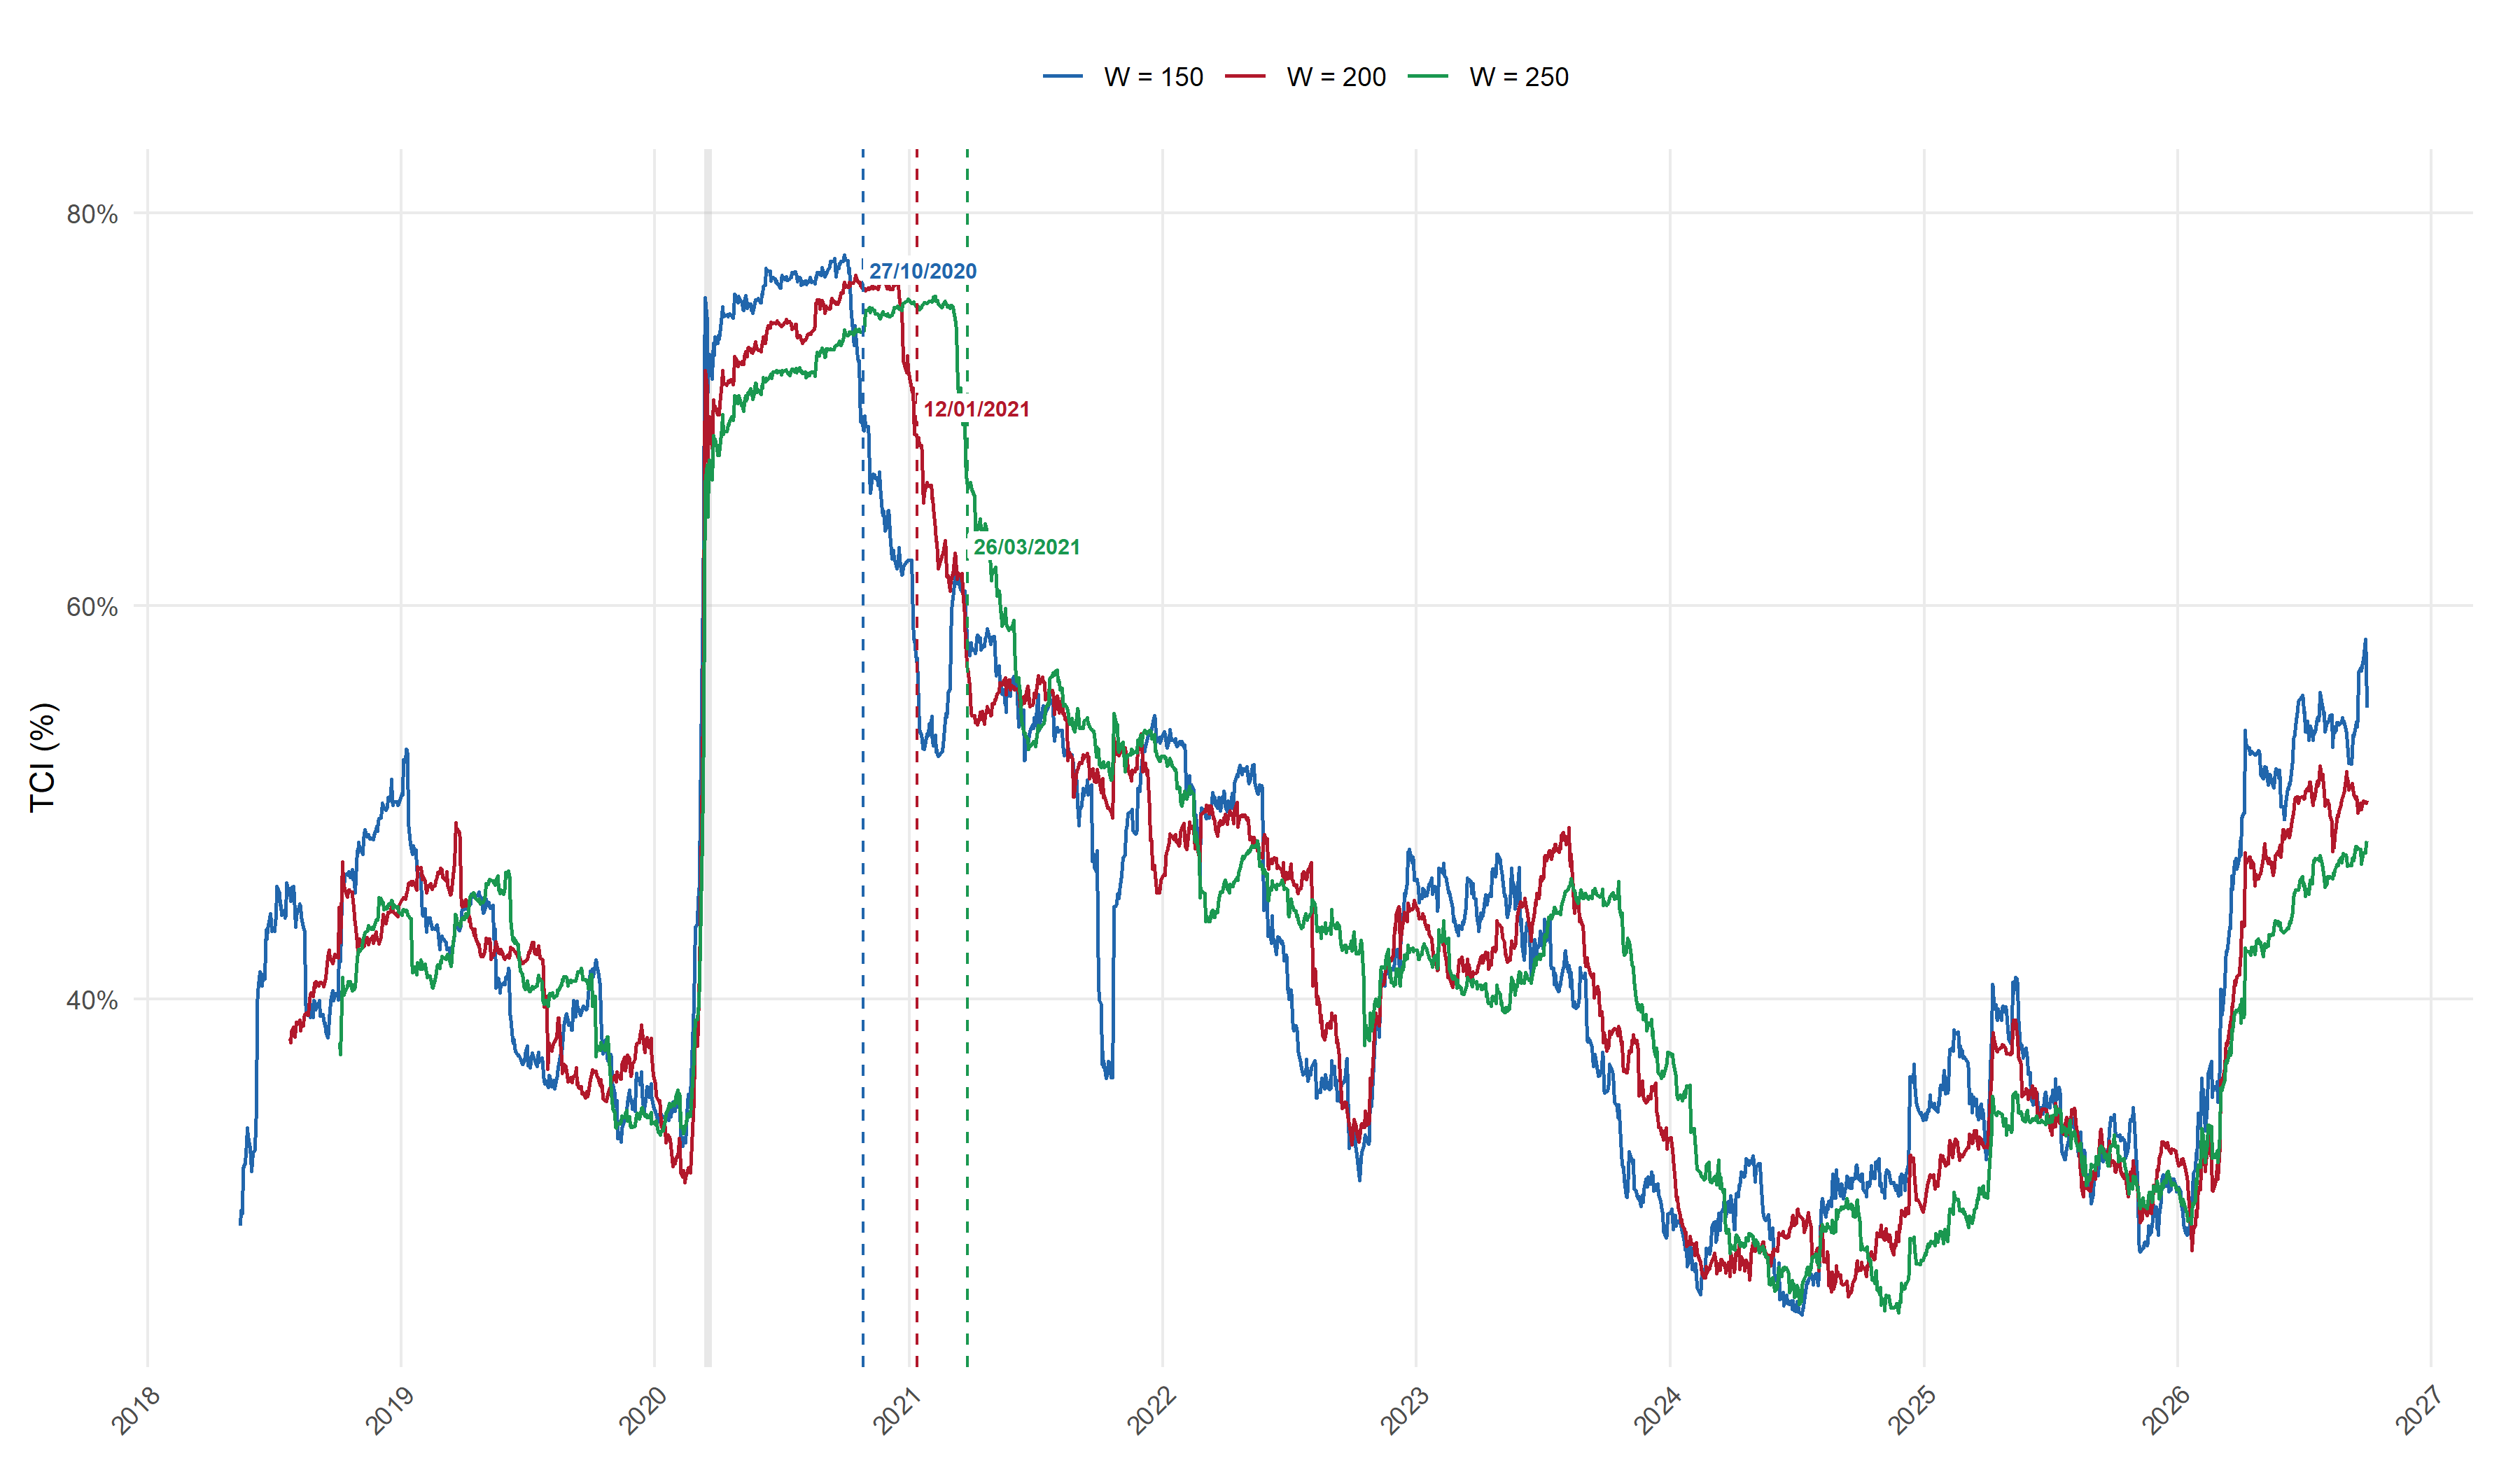
\includegraphics[width=\textwidth]{figuras/tci_comparacao_janelas.png}
  \legend{Fonte: elaboração própria. Linhas verticais: data em que o colapso de
  março de 2020 sai de cada janela.}
\end{figure}

\chapter{Robustez}
\label{ap:robustez}

A Tabela~\ref{tab:robustez} reporta o TCI sob variações do número de defasagens, do
horizonte da decomposição, dos fatores de esquecimento e da subamostra. O nível do
índice varia com a especificação: cai com $p$ (de 53,9\% a 49,3\% no painel principal e
de 57,4\% a 50,4\% no de extensão, entre $p=1$ e $p=4$) e sobe com o horizonte. A
identidade dos extremos, porém, não depende dela. O Itaú é o maior transmissor líquido
nas 13 especificações de cada painel. O Banrisul é o maior receptor líquido em 12 delas
no painel principal e em 11 no de extensão, as exceções são o ABC Brasil na segunda
metade da amostra, nos dois painéis, e o Pan na primeira metade, no painel de
extensão.

A sensibilidade aos fatores de esquecimento é avaliada no par selecionado,
$(\kappa_1, \kappa_2) = (0{,}995;\ 0{,}99)$, e nos pares vizinhos na grade,
$(0{,}99;\ 0{,}99)$ e $(0{,}995;\ 0{,}96)$. A escolha dos vizinhos segue um critério
de proximidade na grade, e não a ordenação por peso posterior, uma vez que, fora dos
dois primeiros pares, todos os pesos são numericamente nulos. O TCI médio varia, em
relação ao par selecionado, 0,9 e 0,4 ponto percentual no painel principal e 0,4 e 0,6
no de extensão.

\begin{table}[H]
\centering
\caption{TCI por especificação}
\label{tab:robustez}
\small
\begin{tabular}{llcc}
\toprule
Variação & Especificação & Principal & Extensão \\
\midrule
Defasagens ($\tau=10$) & $p=1$ & 53,85 & 57,43 \\
                       & $p=2$ & 52,86 & 55,71 \\
                       & $p=3$ & 51,05 & 53,13 \\
                       & $p=4$ & 49,33 & 50,44 \\
\midrule
Horizonte ($p=2$) & $\tau=5$  & 50,17 & 51,72 \\
                  & $\tau=10$ & 52,86 & 55,71 \\
                  & $\tau=15$ & 53,24 & 56,54 \\
                  & $\tau=20$ & 53,30 & 56,73 \\
\midrule
Fatores (TCI médio do TVP-VAR) & $(0{,}995;\ 0{,}99)$ & 50,44 & 52,83 \\
                               & $(0{,}99;\ 0{,}99)$  & 49,55 & 52,40 \\
                               & $(0{,}995;\ 0{,}96)$ & 50,07 & 52,20 \\
\midrule
Subamostra & Primeira metade & 56,60 & 60,91 \\
           & Segunda metade  & 39,19 & 38,09 \\
\bottomrule
\end{tabular}
\legend{Fonte: elaboração própria. Subamostras: 03/10/2017 a 11/04/2022 e 12/04/2022
a 30/09/2026 (painel principal); 03/01/2019 a 27/05/2022 e 30/05/2022 a 13/10/2025
(painel de extensão).}
\end{table}

\chapter{Redes por subperíodo: painel de extensão}
\label{ap:redes}
 
A Figura~\ref{fig:rede-subperiodos-n8} repete a Figura~\ref{fig:rede-subperiodos} para o painel
de extensão, que inclui o Banco Pan. Os subperíodos, a estimação e o limiar são os mesmos; as
posições dos nós são as da rede da amostra completa do painel de extensão
(Figura~\ref{fig:rede-n8}).
 
\begin{figure}[H]
  \centering
  \caption{Rede líquida de conectividade por subperíodo (painel de extensão)}
  \label{fig:rede-subperiodos-n8}
  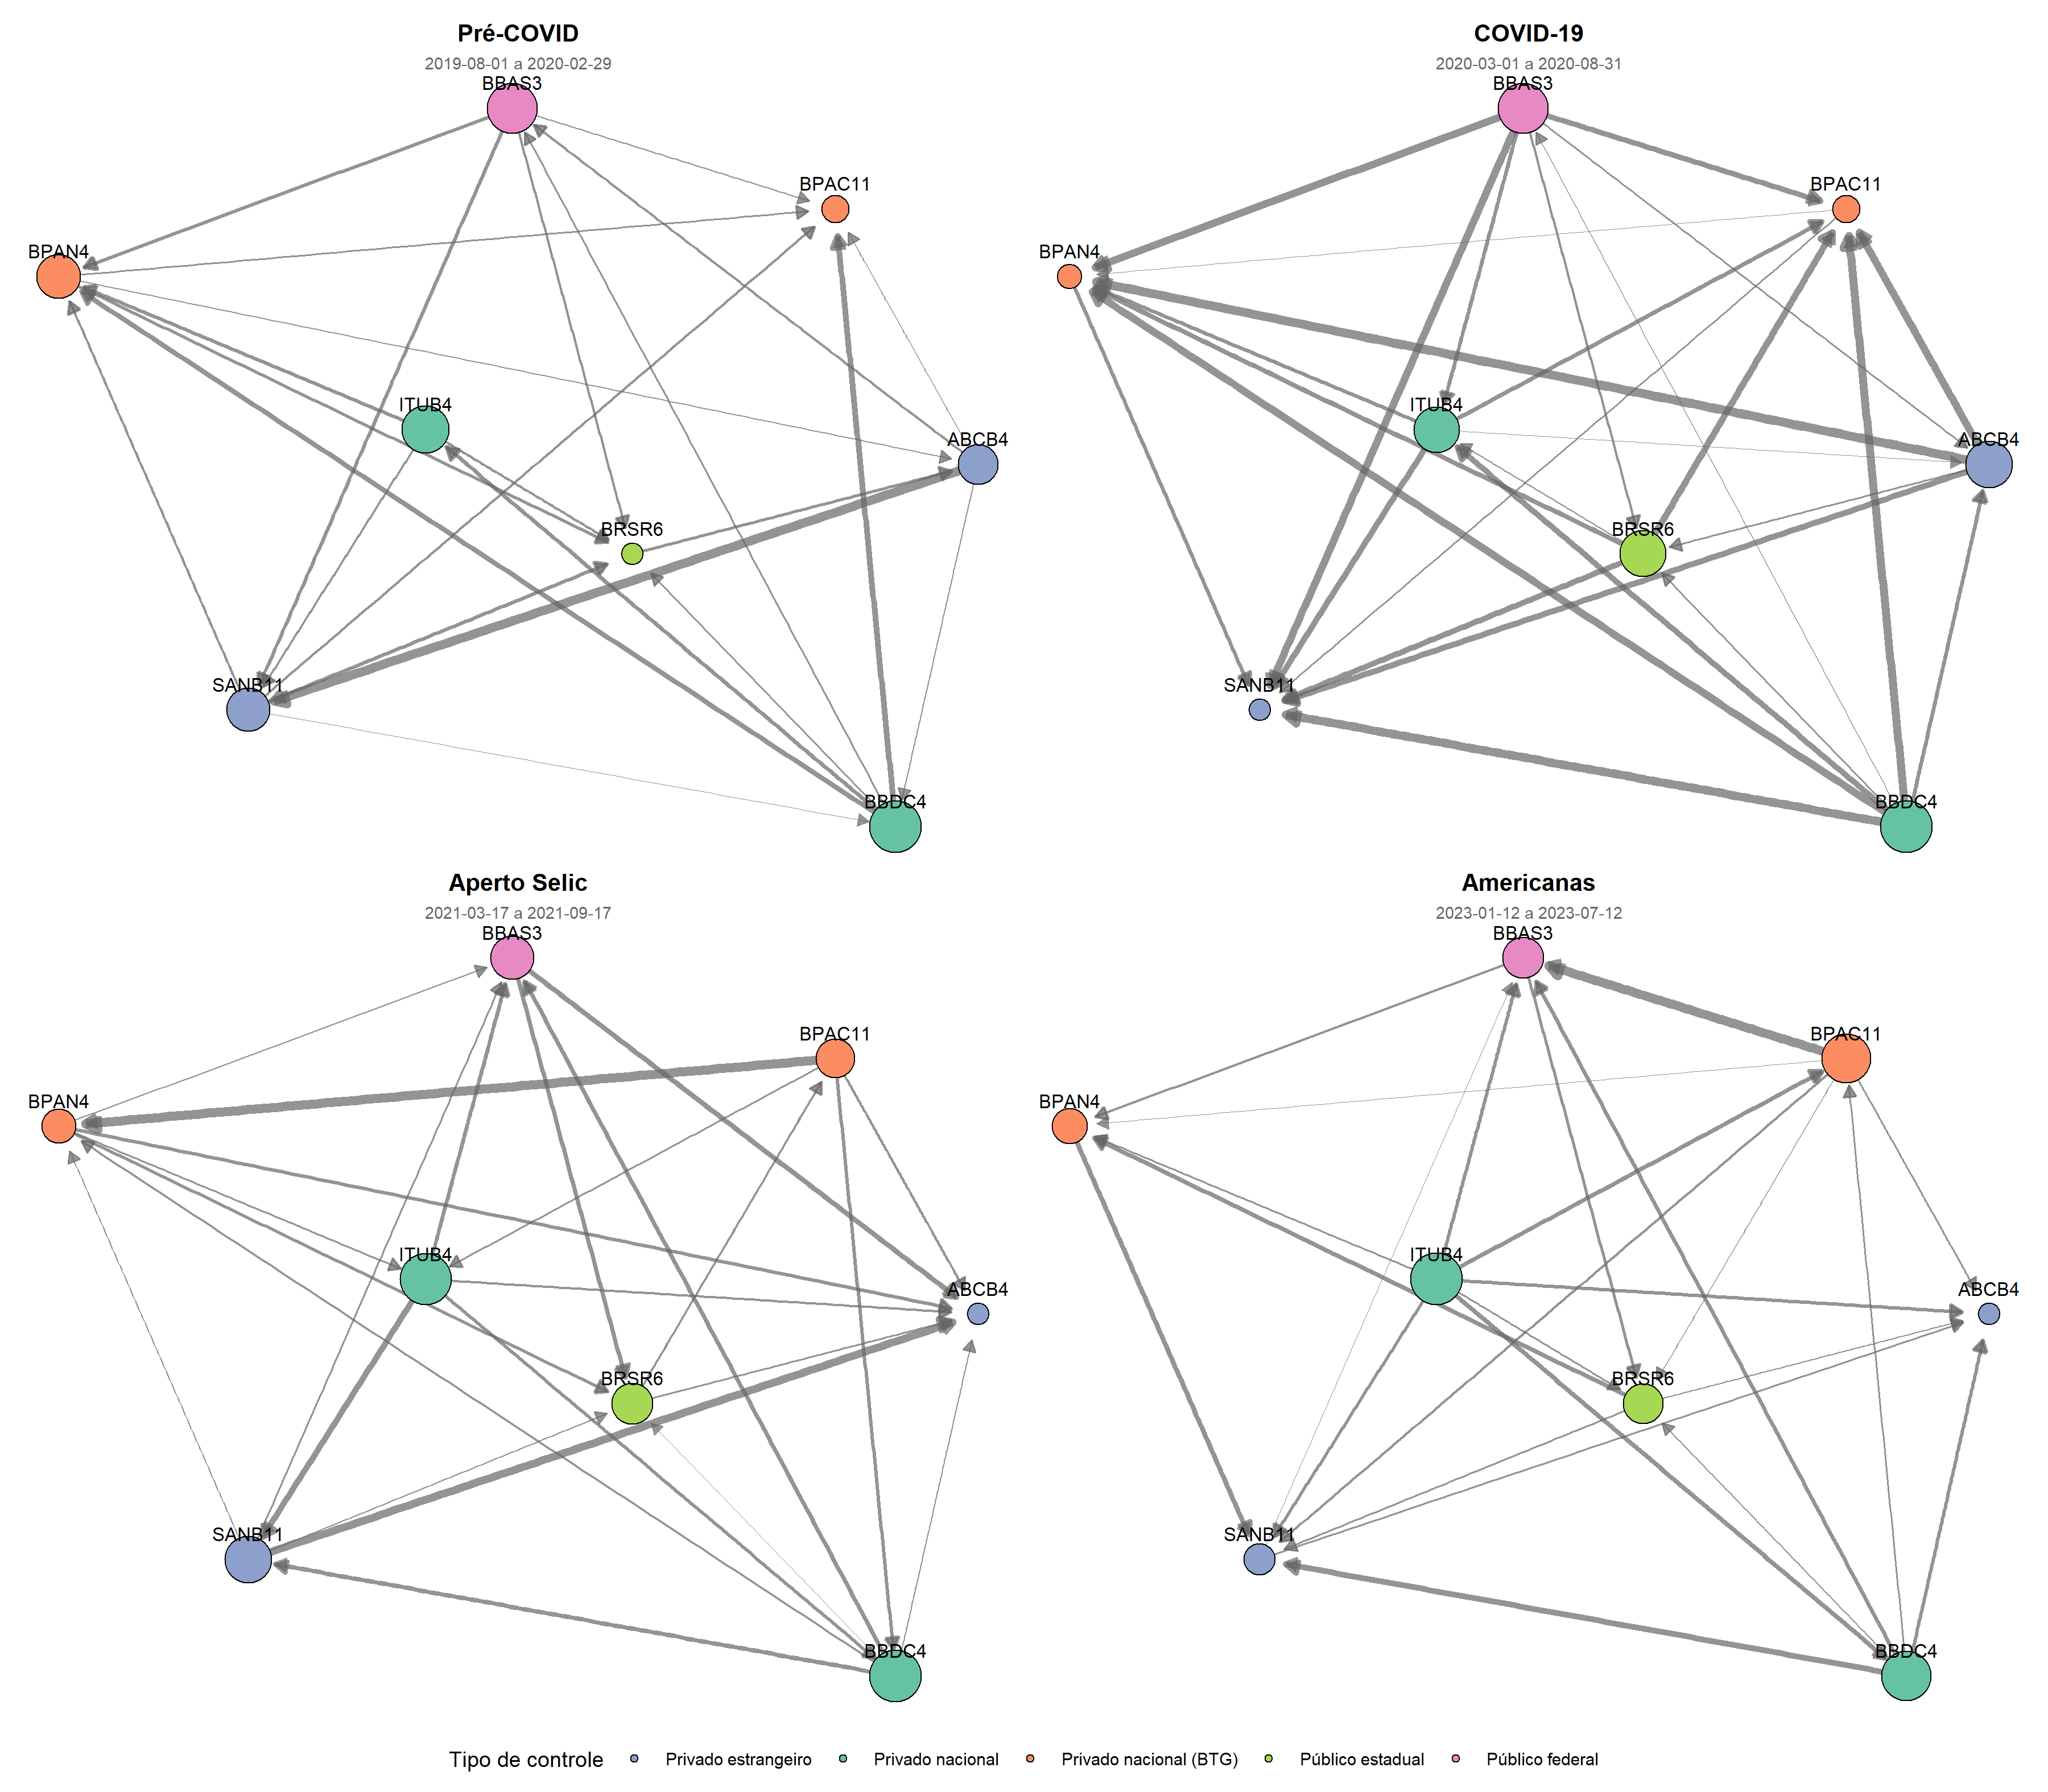
\includegraphics[width=\textwidth]{figuras/rede_n8_subperiodos.png}
  \legend{Fonte: elaboração própria. VAR(2) estático e GFEVD ($\tau=10$) estimados em cada
  subperíodo; limiar de 5\% do par mais forte de cada subperíodo. Posições dos nós fixas, as
  da amostra completa do painel de extensão.}
\end{figure}